% REMEMBER: You must not plagiarise anything in your report. Be extremely careful.

\documentclass{l4proj}

%
% put any additional packages here
%

\begin{document}

%==============================================================================
%% METADATA
\title{Level 4 Project - Type Checker for Dynamic Languages}
\author{Kalok Chan}
\date{April 2021}

\maketitle

%==============================================================================
%% ABSTRACT
\begin{abstract}
\emph{Python}, a dynamically typed language provides an extensive, versatile library of modules for programmers. And due to its forgiving syntax it is the recommended language for beginners. However, this forgiving syntax also causes problems, as \emph{Python} does not perform type checks when compiled. This more evident when programmers are developing in more primitive coding environments. So a static analyser was created as a solution. The analyser is capable of working in and out with IDEs. It is also able to identify data conflicts present code in modules and can accurately report these conflicts. Results show that the analyser developed had a linear scalability in terms of performance relative to the code base size.
\end{abstract}

%==============================================================================

% EDUCATION REUSE CONSENT FORM
% If you consent to your project being shown to future students for educational purposes
% then insert your name and the date below to  sign the education use form that appears in the front of the document. 
% You must explicitly give consent if you wish to do so.
% If you sign, your project may be included in the Hall of Fame if it scores particularly highly.
%
% Please note that you are under no obligation to sign 
% this declaration, but doing so would help future students.
%
%\def\consentname {My Name} % your full name
%\def\consentdate {20 March 2018} % the date you agree
%
\educationalconsent


%==============================================================================
\tableofcontents

%==============================================================================
%% Notes on formatting
%==============================================================================
% The first page, abstract and table of contents are numbered using Roman numerals and are not
% included in the page count. 
%
% From now on pages are numbered
% using Arabic numerals. Therefore, immediately after the first call to \chapter we need the call
% \pagenumbering{arabic} and this should be called once only in the document. 
%
% Do not alter the bibliography style.
%
% The first Chapter should then be on page 1. You are allowed 40 pages for a 40 credit project and 30 pages for a 
% 20 credit report. This includes everything numbered in Arabic numerals (excluding front matter) up
% to but excluding the appendices and bibliography.
%
% You must not alter text size (it is currently 10pt) or alter margins or spacing.
%
%
%==================================================================================================================================
%
% IMPORTANT
% The chapter headings here are **suggestions**. You don't have to follow this model if
% it doesn't fit your project. Every project should have an introduction and conclusion,
% however. 
%
%==================================================================================================================================
\chapter{Introduction}

% reset page numbering. Don't remove this!
\pagenumbering{arabic} 

\section{Motivation}
\emph{Python} is an example of a dynamically typed language which provides an extensive, versatile library of modules for programmers to use. It is also considered as a very intuitive programming language due to its readability, hence the recommendation of being a beginner coding language. However, since \emph{Python} has very lenient syntax, this can produce issues for programmers, new and experienced alike. As \emph{Python} being a dynamically typed language, it does not require users to specify data types of variables, thus when source codes are executed, the execution can potentially be interrupted as a result of the types not being checked. This can frustrate programmers as they are only able to debug one error at a given time due the execution being interrupted whenever it detects an error. Hence, any potential errors in the source code would not be highlighted until the current bug is found and fixed. Some integrated development environments (IDE) already possess some features to mitigate this such as \emph{Pycharm}. However, for programmers that work with \emph{Python} scripts in environments where an IDE is likely unavailable, for example, in a linux headless server, they would need to resort to other script editors say \emph{Vim}. And since such quality of life features are not accessible in such primitive environments, the scripts would are likely to encounter errors thus extending the already long debugging session. 


\section{Aim}
The aim of this project is to assist programmer's coding skills and to allow them to work more efficiently by developing a static analyser which provides an evaluation of their code. The analyser would function in and out with IDE settings. Identify potential data type conflicts for the dynamically typed language, \emph{Python}, will be the primary feature of the analyser. The kind of data type conflicts the software would examine for are:
\begin{itemize}
    \item Inconsistent data type between the same variable.
    \item Incorrect usage of functions, ie providing wrong data types for function.
    \item The components of binary operation.
\end{itemize}

When the software detects all the conflicts found in the source code, it would produce a report informing users what was determined as a conflict, while also explaining why the system has determined it as a conflict.

%==================================================================================================================================
\chapter{Background}

\section{Type Checkers}
\label{sec: what type checker}
Type checkers, one of the many analysis tools, computer scientists uses while they develop their programs. A tool compromising a set of rules ensures that various constructs, such as variables, functions, expressions, or modules, have an appropriate type associated with them. The main objective of type checkers is to verify the data types assigned to these constructs match their expected usage, ensuring that they are type-safe \cite{objective}. Consequently, reducing the possibilities of bugs existing in programs increases the program’s reliability. For example, a function method to calculate the product of two integers. However, two string values were passed as arguments instead, resulting in an error because the function produced unexpected return value. When the type checker flags a program as not type-safe, there is no universal defined process to resolve them. Many programming languages alerts the type errors and terminates the execution or the compilation of the program, while others perform pre-defined countermeasures to handle the errors and maintains the execution\cite{type_check_def}. This however, allows programmers to inherit poor programming practices. As type checking can be performed either at compile time or during run time, there are also two main methods of type checking: static and dynamic.

\subsection{Types of type checker}
Static type checking is when the check occurs at compile time. Such checker requires programming languages to enforce programmers to declare the data types of their constructs before using them. These are primarily used by statically typed programming languages such as \emph{Java} and \emph{C++}. The advantage of applying the static type check is it can identify most type errors early on in the development phase which often makes it more straightforward to debug. The result of this allows the compiled code to be more resource efficient (uses minimal memory) since the data types are known at compile time producing a more optimized machine code \cite{S/D_checking}. Dynamic type checking, on the other hand, is performed at run time. Programming languages that use dynamic type check does not require the programmer to specify the data type before execution, allowing the constructs to be more flexible and beginner-friendly. However, this means that even though the source code is compiled, it is more prone to encountering unexpected errors at run time. \emph{Python} and \emph{Ruby} are a couple of examples of this typed language.

\section{Static Analysis}
Static analysis is the term used for tools that analyse a piece of software without the execution (static) of the application. They are often used to identify:

\begin{itemize}
    \item performance issues
    \item invalid language syntax
    \item Security Vulnerabilities
\end{itemize}

Static analysis is typically performed by automated tools. They are generally used in the early stages of software development to reduce the potential bugs found later on during production. In doing so, the overall production process is increased as debugging became easier due to a lot less code in the code base early on, thus implying less costly for developers to fix the problems \cite{stat2}. The advantages of using such tools are analysis are performed at a quicker rate due to the process being automated as to manually analysing. Another advantage is providing users with more in-depth code analysis during development, allows for greater insight of potential problems. There are disadvantages to using these tools, though, as they may produce false positives/ negatives in the results due their heavy dependence on code patterns and unable to adapt to understand the user's intent within the given context. 


\section{Abstract Syntax Tree}
An abstract syntax tree (AST) is a tree representation of the source code of a program to illustrate the structure of the code \cite{ast}. When a source code is parsed to create an AST, only the structure and the constructs of the source code are preserved. The preserved code is then used to produce a hierarchical tree where all nodes represent the components of a construct. An example is shown on Figure \ref{fig:ASTB}.

\begin{center}
    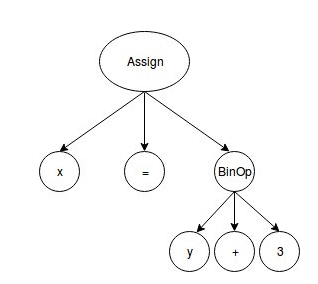
\includegraphics{images/ASTB.png}
    \captionof{figure}{An simple AST representation of the \emph{Python} code: x = y + 3 Source: \cite{ASTBasic}}
    \label{fig:ASTB}
\end{center}

ASTs are often used in static code analysis, which is the process of analysing a program for problems ie syntax errors or vulnerabilities in the code without the actual execution of the program.

\section{Related research}
The following section is about current static analysers the are currently available and is used by many programmers and past researches conducted on type checkers.

\subsection{Mypy}
\label{sec:mypy}
Mypy  \cite{mypy} is a static type checker developed for \emph{Python}. It makes use of \emph{Python's} annotation syntax, type hints, to perform type checks of programs and find common bugs. Type hints are a set of annotation that acts in the same way as comments where it informs the programmer more about the code but does not actually contribute to the execution of the program. It is used in a similar fashion as how \emph{Java} defines its method definitions, as shown on Listing \ref{lst:java} and \ref{lst:python}. 

\begin{lstlisting}[language=Java , caption= Java function definition, label={lst:java}]
public boolean isOdd (int number):
\end{lstlisting}
\begin{lstlisting}[language=Python, caption= Python function definition with type hints, label={lst:python}]
def isOdd (number:int) -> bool:    
\end{lstlisting}

Mypy is designed as sort of a bridge between dynamic and static typed languages. This is because Mypy only performs the type checks when type hints are present in the source code, allowing programmers to return to the basic dynamic typing when static typing is not feasible. However, this implies that users are required to learn how to code type hints properly to be able to benefit the feature Mypy provides.

\subsection{Pyflakes}
\emph{Pyflakes} is also a static analyser developed for \emph{Python}. Its design concept ignores coding styles, but ensures that false positives almost never occur during their code analysis. Since it only ever analyse logistic errors \cite{stat}, it is very limited in what the analysis can detect compared to the other static analysers. The trade off for this is than its much faster than \emph{Pylint} and \emph{PyChecker}, since it verifies each file individually. 


\subsection{Type Checkers via Slice \& Run}
Adam and Kell \cite{A&K} discusses the novelty idea of the ability to evaluate advanced type invariants and properties in source codes while maintaining the speed and simple usage of the conventionally available syntax-directed type checkers. To achieve this, they have proposed an alternate method of evaluating static type checking through the use of symbolic execution along with “type assertions”. However, to tolerate the awful scaling and under approximation of symbolic execution, a reduced portion of the program is derived, utilizing program slicing that slice with respect to certain criteria. 


%==================================================================================================================================
\chapter{Analysis/Requirements}

As mentioned in \hyperref[sec: what type checker]{chapter 2}, \emph{Python} is a weakly-typed language, thus constructs are more flexible in that their initial data types can be overwritten by different data types, intentionally or not. This makes it difficult for users to track the types and more prone to encountering type conflicts. Hence the requirements of the final software are derived from the functionality of a typical static type checker to mitigate this. The functionalities can be summarised in, the ability to identify potential data conflicts and highlight such conflicts to assist users in debugging their code.

The strongly typed \emph{Java} programming language was used to determine what kind of data conflicts the software would check for. This was done by locating where users would need to declare a data type for a given construct. Then identify which of these constructs are more likely to be given a different data type during the development thus resulting a type error. Consequently, the concluded data type conflicts the software would check for are as follows:

\begin{itemize}
    \item The data type consistency of a variable within its scope
    \item Binary operations on unsupported data types
    \item The data type consistency of the arguments of a method call with respect to its function signature 
    \item Object method calls are within scope of the class definition
\end{itemize}

After the type checks are performed, a report shall be produced. This will consist of a list of defined constructs with their last known data type along with the code line it was last used in. It will also report all data conflicts found and on which line and construct did the conflict occurred in.

These requirements are then prioritised using the MoSCoW method \cite{moSCoW}, a method of prioritisation, which categories the requirements into four headings:
\begin{itemize}
    \item \textbf{Must Have:} features which are critical to the program and without it the program will not function.
    \item \textbf{Should Have:} features which are essential to the program but not critical, meaning the program will still function without it but is less usable.
    \item \textbf{Could Have:} features which are desirable to the program but can be excluded if time and resources do not permit.
    \item \textbf{Would Not Have:} features which have little impact to the program and will not be present in the program.
\end{itemize}
This is used to illustrate the importance of each requirement and to determine which requirement was viable within the time frame.

\clearpage
\section{Functional Requirements}
These requirements are features that describes the functionality of the system. 

\subsection{Must Have}
\begin{itemize}
    \item \textbf{Converting source code to an AST:} This provides the program the ability to analyse source code and search for specific constructs allowing the program to perform the required type checks for the constructs.
    \item \textbf{Determine the data type of a variable:} The fundamental feature of the program as this allows the program to inspect the data type of a variable which is then applied to perform the type checks.
    \item \textbf{Data type consistency between variables:} The type check performed to ensure that initialised variables have a consistent data type throughout its scope. As this is the most common data type error programmers encounter where they thought one variable is one data type but in actuality, it is another data type.
    \item \textbf{Report:} A summary of the results performed from analysing the source code.
\end{itemize}


\subsection{Should Have}
\begin{itemize}
    \item \textbf{Data type consistency between components of Binary Operations:} The type check performed to ensure the components of the binary operations have similar data types for example integer to integer and integer to float etc. While also flagging invalid or unsupported operands such as string subtracting a string.
    \item \textbf{Validity of method calls:} The type check performed to ensure the data type of components of arguments are of the expected type found in the function parameters.
\end{itemize}

\subsection{Could Have}
\begin{itemize}
    \item \textbf{Class Object Compatibility:} The ability to perform type checks mentioned above with class objects.
    \item \textbf{Scope of Object Method Calls:} Class object method check to ensure method calls are within the scope of the class.
    \item \textbf{Provide recommendations to type conflicts found:} When a conflict is detected the program would provide possible solutions to resolve the conflicts found in the source code.
\end{itemize}

\section{Non Functional Requirements}
The non functional requirements relate to the properties of the system.

\subsection{Quality of service}
\begin{itemize}
    \item The system is responsive and results produced in milliseconds 
    \item The system has good scalability 
    \item The systems analysis is accurate
\end{itemize}

\subsection{Availability}
\begin{itemize}
    \item The system is intuitive and can be used easily by both new and experienced programmers
    \item The system works on all modern computers
    \item The system works in and outwith IDEs
\end{itemize}

%==================================================================================================================================
\chapter{Design}

Before developing the code base for the system, the general behaviour of the system had to be determined. This was to help identify what sort of functions the system required to perform the static analyses while also providing a general idea of the order of implementation. A Flow diagram was created to help visualise this, as shown in figure \ref{fig:UML}.

\begin{center}
    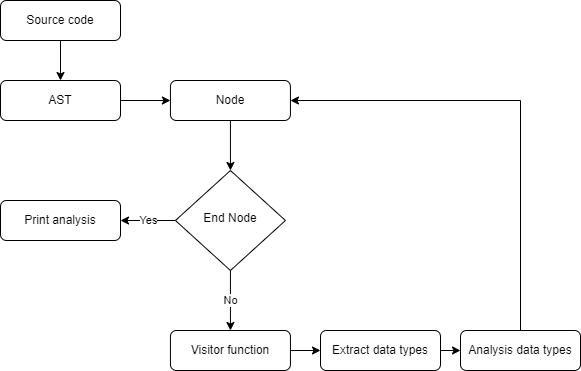
\includegraphics[width=\textwidth]{images/UML_activity.png}
    \captionof{figure}{flow diagram of general behaviour of the static analyser}
    \label{fig:UML} 
\end{center}

From the diagram we can observe that the system should start from creating an AST from the provided source code. The nodes are then iterated through while visiting the appropriate visitor function associated with that node type to process its data. More detail about the visitor functions in the Subsection \hyperref[sec:visit]{Visitor functions}. Afterwards, from the processed data, the analyser would then extract the data types and compare it to the data type of the same variable name, if it exists. This process is repeated until the all nodes in the AST has been traversed at least once. Finally a report will be generated from the analysis and is provided for the user to evaluate.

\section{Abstract Syntax Tree}
As the objective of the system is to perform an analysis on a given source code, it is clear that code will need to be parsed before any analysis can be performed. Hence, the function that creates the abstract syntax tree is after the source code near the top of the diagram as it is the first process that the system preforms after being provided with a source code to analyse. So, users are prompted to first specify which code module they would want a static analysis to be performed on. The module could consist of assignments, functions, class objects and also built-in modules provided by \emph{Python}. The AST created is a tokenised representation of the code base meaning that each node is of the language syntax ie an operator, data literal, variable name etc. For example, a \emph{Python} representation of the Euclidean algorithm, Listing \ref{lst:ast}, would have an AST created similar to the one shown in Figure \ref{fig:AST}. Afterwards the tree is traversed by starting from the name of the module also known as the root node of the AST, to each node representing different sequence statements of the body of the module then iterating down depth first until the child node is reached before exploring the neighbour nodes. In this example, the system would traverse the left child first in other words the compare node then variable and constant before iterating down the body branch.

\begin{lstlisting}[caption= A \emph{Python} representation of the Euclidean algorithm adapted from wikipedia \cite{astcode}, label={lst:ast}]
while b != 0:
    if a > b:
        a = a - b
    else:
        b = b - a
return a
\end{lstlisting}

\section{Visitor Functions}
\label{sec:visit}
The objective of each traversal of the nodes is to recognise code patterns within the module where possible type problems can occur. Visitor function are exploited to accomplish this task. The purpose of these functions is once identified, the system will attempt to parse the data provided into a specified form so that their data types can be extracted using the extraction function.

\subsection{Assignment}
The assignment visitor function would be the most common function visited as variable assignments have the most frequent appearance within code bases. The purpose of this visitor is to differentiate between whether the variable assignment made is a method call or just a assignment to a data structure. When it is the latter, then it will be parsed for the extraction function. Whereas the \hyperref[call]{Call visitor function} is initiated when a method call is determined. 
 
\subsection{Function Definition}
When a function definition node is encountered, this visitor function is visited. Its main objective it to parse the node of the data types of its ins/outputs to create a function signature and store it so it can be referenced during the process of determining whether the function is type safe, in other words to identify invalid method calls. Examples of invalid method calls include:
 
 \begin{itemize}
     \item Non existent method calls, in other words a method call to a function that either has not been defined yet or straight up does not exist.
     \item Inconsistency between the call arguments and the defined parameters. 
 \end{itemize}
 
 After successfully creating the function signature, the system would examine the rest of the definition to locate any local variables defined and call the Assignment visitor function to ensure that the definition does not break the type checks defined or to identify other sequence statements nodes and visitor their appropriate visitor function.

\begin{center}
    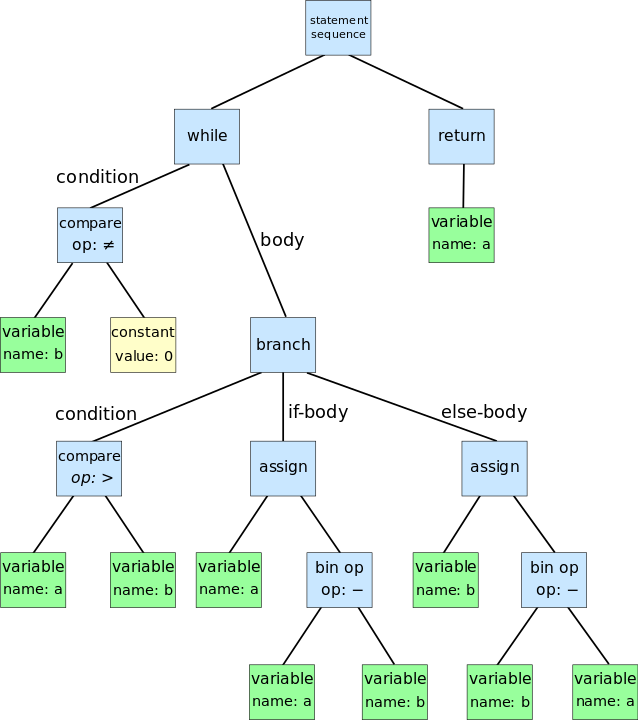
\includegraphics[width=\textwidth]{images/AST_diagram.png}
    \captionof{figure}{An abstract Syntax Tree representation of the Euclidean algorithm to find the greatest common divisor of a and b, Source from Wikimedia Commons \cite{ASTdia}}
    \label{fig:AST} 
\end{center}

\subsection{Call}
\label{call}
The Call visitor is used whenever a method call is initiated. The visitor determines the validity of the method calls by utilising the function signature generated from the function definition visitor. To do this, the function would first verify whether the function of the method call exits. Then check for consistency of the arguments and the parameters before performing a data type analysis on the called function with the data types of the arguments. Finally, the Call visitor would obtain the data type of the return value of the called function with the extraction function and executes a consistency check with the variable assigned to the method call.

\section{Extraction of data types}
This is the function that will determines what method of parsing is required for the assignment nodes to obtain their data types and is where most visitor functions proceed to after completing their objectives. There are three main assignments the function anticipates for:

\begin{itemize}
    \item Binary Operations
    \item Assignment associated with another variable
    \item Built-in Data types
\end{itemize}


In the case of Binary Operations, each components data type will be obtained and performs a check to ensure that their types are consistent and the operation performed is valid for that data type. If the assignment has an association with another variable, the function will ensure that the variable exist before extracting their data type, else it would report the usage of a non existent variable. Finally if the assignment is a built-in data type then their data type is just simply extracted. 

\section{Consistency of data types}
The consistency function as the name suggests, is a function that ensures the data type consistency of variables and is the function that almost all visitor functions end up due to assignments made. It performs the consistency type check by iterating through each variable within the data dictionary that is passed as an argument and compares it with the target variable. When the name of the variables match their data types are verified for consistency and if true then the code line of target variable is used to update the variable in the dictionary. Otherwise, information of the variable is provided to the error recorder that is used for the analysis report.

\section{Analysis report}
Finally once all nodes have been traversed and analysed, the report function is then initiated. This handles the errors analysed by the program during the analysis of the source code. It addresses the variable that caused the conflict, where it occurred and what the reason for the program to flag it as a conflict. By reporting these information it would help the user locate the conflicting type checks. The analysis also provides the user the last known data types of defined variables, function signatures, class definitions and defined object attributes all to ensure that the data type is of the type expected by the user and to assist the user in debugging the conflict. 

%==================================================================================================================================
\chapter{Implementation}
The implementation of the static analyser was developed in the \emph{Visual Studio Code} IDE, written on \emph{Python} version 3.7.5 with the intention of analysing \emph{Python} source code written in version 3 onwards.

\section{Abstract Syntax Tree}
To create the abstract syntax tree for the static analyser, the \emph{Python} module \textit{'AST'} was imported. This module generates the syntax tree by applying the \textit{parse} function provided by the module. By providing the source code as an argument to this function, a tree of objects is returned as a result. These objects inherits the classes of \textit{ast.AST} which are utilised in categorising the nodes from their corresponding \emph{Python} expression. Assign, BinOp, List and ClassDef are a few of such classes.

\section{Extraction}
Many extraction methods were created to enable the function to extract the relevant data from the nodes. This was because even though the ast stores the data in a similar structures for all its classes there is still a slight difference between them. For example, to extract the name of the variable assignment from an binary operation would require the program to access the targets of the node then access the id to obtain the variable name of that assignment, refer to Figure \ref{fig:assign_struct} for an idea of the structure. Whereas, to obtain the same variable name of an assignment to a class attribute, the process is to access the attribute field of targets rather than the id, as shown in Listing \ref{lst:variableName}. 

\begin{lstlisting}[language=Python, caption= Code snippet of extracting the variable name of a node, label ={lst:variableName}]
if not isinstance(node.targets[0], ast.Attribute):
    variableName = node.targets[0].id
else:
    variableName = node.targets[0].attr
\end{lstlisting}

To investigate how to extract relevant data from a node, the function \textit{dump} from the AST module can be used along with the \textit{print} function or using the alternative \textit{astpretty} module\cite{pretty}. Using node as the argument either function, the structure of the node and its relevant data will be printed to the console allowing for analysis just like Figure \ref{fig:assign_struct}.

\begin{center}
    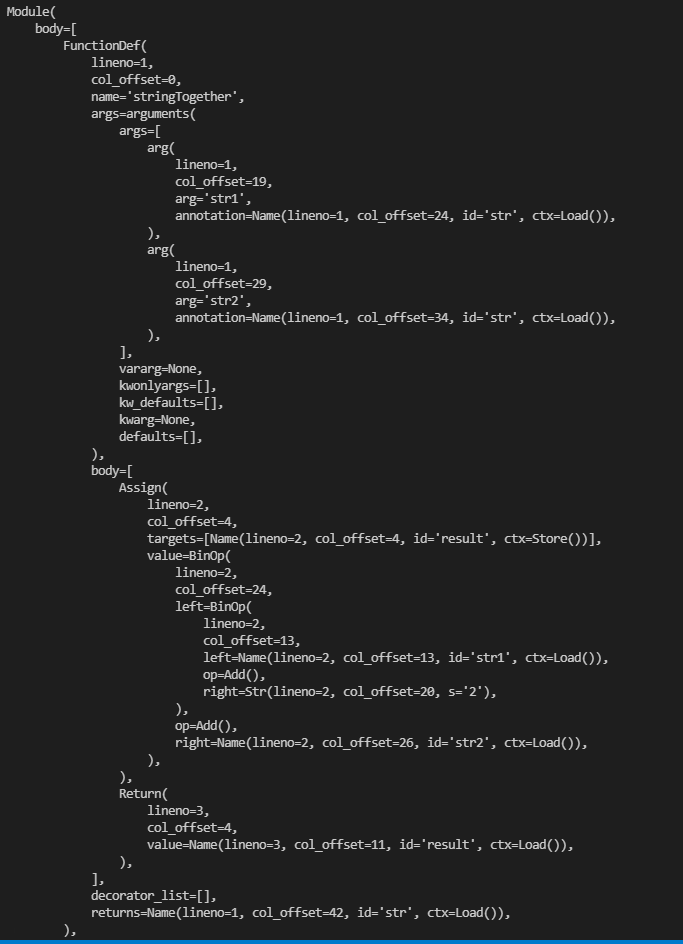
\includegraphics[width=\textwidth,height=\textheight,keepaspectratio]{images/AST_class.png}
    \captionof{figure}{Screenshot of a part of the AST created for the \textbf{withTH.py} module displayed using astpretty module\cite{pretty}. Displays a parsed function node produced by the AST Module, demonstrating what and how the data is stored in the AST.}
    \label{fig:assign_struct}
\end{center}

\clearpage
For all nodes, the data to be extracted are:
\begin{itemize}
    \item the code line at which the node occurs at.
    \item the variable name if it is an assignment node.
    \item the values of the assignment ie the components on the right hand side of the assignment.
\end{itemize}
Once extracted the actual data type of the values can be obtained with the combination of either \textit{type} function with \textit{literal\textunderscore eval} function from the \textit{ast} module or with \textit{eval} function from \emph{Python}'s built-in library. Both \textit{eval} functions work in a similar way, where they both take \emph{Python} literals expressions as arguments and returns the result of the evaluated expression. \emph{Python} literals are defined as the raw data assigned to variables or constants during the development a of software or program which consists of:

\begin{itemize}
    \item String 
    \item Numeric  - Integer, Float, Complex
    \item Boolean 
    \item Collections - List, Tuple, Dictionary and Set
    \item Special - None
\end{itemize} 

From the results of the evaluated expression, \textit{type} function can be used to obtain the data type. However, literals are not the only expressions that the built-in function \textit{eval} can have as an input. As long as the input is a string then function will evaluate that expression regardless of its contents. This shows how powerful this function can be, but also the dangerous implications it has as it can be used to perform system commands. Therefore \textit{literal \textunderscore eval} was opted were possible as the method of extracting the data type of nodes. A quick comparison of the \textit{eval} functions can be seen in Listing \ref{lst:eval}

\begin{lstlisting}[language=Python, caption= Comparison of \textbf{literal\textunderscore eval()} and \textbf{eval()}, label = {lst:eval}]

import ast
ast.literal_eval("{'a': 1, 'b' : 'qwerty', 'c' : 3}")
# output: {'a': 1, 'b' : 'qwerty', 'c' : 3}
ast.literal_eval("__import__('os').system('rm -rf /')") 
# output: error

eval("{'a': 1, 'b' : 'qwerty', 'c' : 3}")
# output: {'a': 1, 'b' : 'qwerty', 'c' : 3}
eval("__import__('os').system('rm -rf /')") 
# output: proceeds to remove files within the specified directory
\end{lstlisting}


\section{Binary Operations}
When approaching the implementation for type checking Binary Operations, it was not as simple as simply using the extract function to obtain the data types of the components and then validate them with respect to the type check rules defined. This is because of how the structure of the Binary Operation node differs when it gets parsed by the \textit{ast} module depending on the number of components within said binary operation. An example of this can be observed on Figure \ref{fig:BinOp}.

\begin{figure}[h]
    \centering
    \begin{subfigure}[b]{0.45\textwidth}
        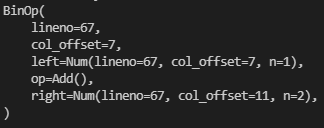
\includegraphics[width=\textwidth]{images/BinOp1.png}
        \caption{Binary Operation with \textbf{two} components}
        \label{fig:Bin1}
    \end{subfigure}
    ~ %add desired spacing between images, e. g. ~, \quad, \qquad, \hfill etc. 
      %(or a blank line to force the subfigure onto a new line)
    \begin{subfigure}[b]{0.45\textwidth}
        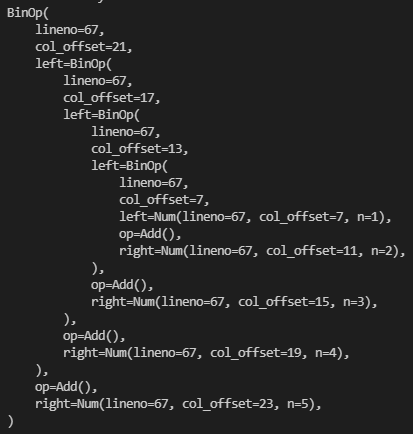
\includegraphics[width=\textwidth]{images/BinOp2.png}
        \caption{Binary Operation with \textbf{five} components}
        \label{fig:Bin2}
    \end{subfigure}
    ~ %add desired spacing between images, e. g. ~, \quad, \qquad, \hfill etc. 
    %(or a blank line to force the subfigure onto a new line)    
    \caption{Output of the \textit{pprint} function displaying the structure of a Binary Operation node. \subref{fig:Bin1} shows the simple structure of just left and right when there is only two components present \subref{fig:Bin2}
    shows a more complex structure of nested values when more than two components are present.
    }\label{fig:BinOp}
\end{figure}

From the Figure \ref{fig:Bin2}, it can be concluded that when a Binary Operation has greater than two components, the structure would begin to nest itself. To tackle this, a recursive function was implemented. The recursive function would repeatedly call itself until it reaches the inner most part 
of the structure before executing the rest of the function as shown in Figure \ref{fig:recursion}.

\begin{center}
    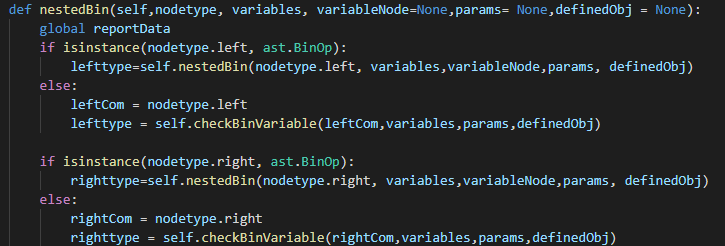
\includegraphics[width=\textwidth]{images/BinRec.png}
    \captionof{figure}{The recursive function implemented to tackle the nested structure of Binary Operations}
    \label{fig:recursion}
\end{center}

The function carries out this recursion by doing a recursive function call whenever it encounters a Binary Operation in the current nodes "left" value. Otherwise it would call \textit{checkBinVariable} to obtain the data type of the node. This is then repeated with the "right" values. Afterwards, it would compare the data types of each component ensuring that they are the same to pass the consistency type check, with the exception of integer and floating point data types. This is due to them being part of the Numeric data type, and are often interchangeable between them, hence when both components are of either type it would pass the consistency check.

\section{Function Definition}
Similar to what was mentioned about \emph{mypy} in section \ref{sec:mypy}, the types of parameters can be obtained using type hints. This is achieved through examining each parameters attributes if the annotations attribute is present. When present, the type hint is extracted and the function \textit{eval} is used to evaluate the data. As specified above, although \textit{eval} can have dangerous implications it can be argued to be safe to use in this situation. This is because the type hints are defined by the programmer of the source code, thus are very unlikely to use system commands as type hints for the parameters of a function. Another reason for using \textit{eval} is, by using type hints programmers are indicating what the data type of a parameter is by directly specifying the types such as str, int, bool etc. However, since actual data types are specified rather than a value of the equivalent data type, they therefore cannot be classified as a \emph{Python} literal. Hence, the extracted data would become incompatible with \textit{literal\textunderscore eval} and would result in errors if attempted. After successfully obtaining the function signature through the use of type hints, type checking is performed for the local variables defined within the function.

Nonetheless, this is only a partial solution to the problem as this requires programmers to possess the knowledge of type hints and the ability to correctly utilize them. Also by using type hints it limits the use cases of a function as each parameter can have only one type hint specified. For example, if the programmer wanted a function that requires two of the same collection data structures, such as list or tuples, as the input and returns an extended version by appending those two together, then they would need perform a polymorphism of overloading the function. This is the concept of creating multiple functions of the same name with the similar functionality but has different data types for parameters (function signatures), visualised in Listing \ref{lst:poly}. However, this concept not applicable to \emph{Python} since it is a weakly typed language, so types do not need to be specified. Hence instead it would simply override the functions defined earlier with the latest one. So to maintain the ease of use and parameter flexibility \emph{Python} has a \textit{hints} variable is introduced to the function signature. If type hints are present then the analyser would store the parameters along with their data types in the function signature variable with the \textit{hints} variable set to true. Else, the variable is set to false and only the names of the parameters are stored. In the case of return, if the value cannot be obtained when the function is defined due to the lack of type hints then the variable is stored instead of the actual data type.

\begin{lstlisting}[language=Python, caption= Example of overloading functions (Polymorphism), label = {lst:poly}]

# functions with the same name but has different function signatures
def extend(data1:list, data2:list) -> list:
    return data1+data2
    
def extend(data1:tuple, data2:tuple) -> tuple:
    return data1+data2
\end{lstlisting}

\section{Call}
Before performing the consistency type check of arguments and function parameters, the name of the method call needs to examined to ensure that it has been defined. This is done with the assistance of the helper functions \textit{getFuncName} and \textit{returnLookUp}. As the name implies, \textit{getFuncName} returns the name of the method call and if the call was an object method call then it returns a tuple of the object class, the function name and the name of the object. The returned function name is then checked whether they are user-defined functions or is an object method call. When it is neither of those then the \textit{returnLookUp} is used to examine the possibility that the function call is a built-in function or an object creation call. In the instance that the name is not found by the \textit{returnLookUp}, then a non existing function error is raised and the variable of the method call is assigned the value \textit{None}. If it is a built-in function then only the return type will be type checked for consistency as all built-in functions return types are all predetermined. Otherwise the consistency type check of arguments and function parameters will be performed.

Due to allowing programmers the ability to define functions either with or without type hints, two separate methods are required to type check function inputs, \textit{callHints} and \textit{callNoHints}.

\subsection{With Hints}
When functions are defined with type hints then process is much simpler. As all data types of the ins and outputs of the function is known beforehand, they can be obtain by simply accessing the function signature variable. For the data types of arguments, they are obtained through a similar method to extraction except when variables are passed as arguments then the data type is obtained by searching through the \textit{variableList} variable containing initialised variables. Afterwards it is as straightforward as comparing the two data types for consistency, as shown in Figure \ref{fig:callHint}. A note regarding method calls are, arguments can have the keywords syntax so arguments do not need to be passed in order with regards to the function signature, an example shown in Listing \ref{lst:keywords}. So to deal with this, the function checks for keywords present before proceeding to analyses the types. When they are not present then the consistency type check is between the data types in the same position in the function signature and the method call. Otherwise the keyword is matched with the parameter variable before type checking them.  

\begin{center}
    \includegraphics[width=\textwidth]{images/callHint.png}
    \captionof{figure}{A code snippet of \textbf{callHints} that type checks the consistency of method call inputs without keywords.}
    \label{fig:callHint}
\end{center}

\begin{lstlisting}[language=Python, caption= Method calls with/out keywords showing that order does not matter when keywords is used as the function still works, label = {lst:keywords}]

def stringTogether(str1, str2):
    result = str1 + "2" + str2
    return result
    
a = stringTogether("hello", "world")
# a has the value "hello2world"

b = stringTogether(str2= "hello", str1= "world")
# b has value "world2hello"

\end{lstlisting}
\subsection{Without Hints}
Since functions without type hints has no data types for their parameters in the function signature, a full type check was not performed during the function definition stage as functions that use their parameters for some execution of code their data types are unknown. Thus, an almost different approach to type check the validity of the method call is required. Instead of performing a type check between the arguments and the parameters, a new variable \textit{Nparam} is created which stores the parameters with the updated data types provided by the arguments, as shown on Figure \ref{fig:Nparam}. This is then used along with the \textit{revisit \textunderscore method} helper function, to perform a full type check analysis as all variables used in the function is now known. The \textit{revisit \textunderscore method} function is a function that, provided a target function name and a parameter list, would search through the AST for said target node and performs an type analysis while extending the parameter list with the local variables defined within the function. The parameter list is extended so that if the return type of the function uses the local variables defined, the data type can be obtained and used for consistency type checking for the variable that is assigned to the method call.

\begin{center}
    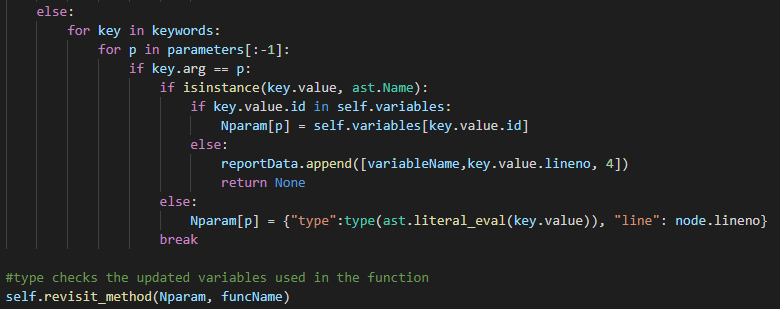
\includegraphics[width=\textwidth]{images/Nparam.png}
    \captionof{figure}{A code snippet of \textbf{callNoHints} of how the variable \textit{Nparam} is obtained when keywords are used in the method call and how it is utilised.}
    \label{fig:Nparam}
\end{center}

\subsection{Nested method calls}
As with how the binary operation structure can be nested when it gets parsed by the \textit{AST} module, method calls can also be nested. This occurs when a function calls is initiated within a function definition. Hence, the call visitors function signature had to be extended to include parameters with default values to tackle this. Listing \ref{lst:call} visualises the function signature accompanied with comments regarding each parameter.

\begin{lstlisting}[language=Python, caption= Function signature of the \textbf{Call} visitor,  label = {lst:call}]
def Call(self, node,variableList, NestCall = False, NestArg= None, variableName = None, initial = False):
# node: containing all data relevant to the method call
# variableList: either the global variable list or the local variables of the function that contains a nested call
# NestCall: boolean field used to verify whether the method call is a nested one or not
# NestArg: arguments of the nested call or the function signature of the current function that contains the nested call
# variableName: name of the variable which initiated the nested call
# initial: boolean field verifies whether the visitor is initiated during a function definition or due to an assignment method call outwith the definition
\end{lstlisting}

\clearpage
With the extra information obtained through the extended parameters, the helper functions \textit{callHints} and \textit{callNoHints} are able to to handle the nested calls appropriately. As shown in Figure \ref{fig:callHintN}, when nested call initiated by the initial function definition stage, it is handled in a similar fashioned as to without nested calling, Figure \ref{fig:callHint}. The exception is the additional code from \textit{360-370} where the first \textit{elif} statement handles the arguments data types if the parent function uses type hints. The other \textit{elif} statement occurs when the parent function does not use type hints and instead assigns the argument with 'TBC', this is used to bypass the consistency check since the data types are physically impossible to obtain when it is being defined. However, it will be replaced and type checked when actual data with data types are passed to the function with the nested call. It can also be observed that when the nested call is not an "initial" one then the type check is as simple as obtaining the data type and comparing it with is corresponding parameters type. This process also applies to \textit{callNoHints} but with the no hints equivalent.

\begin{center}
    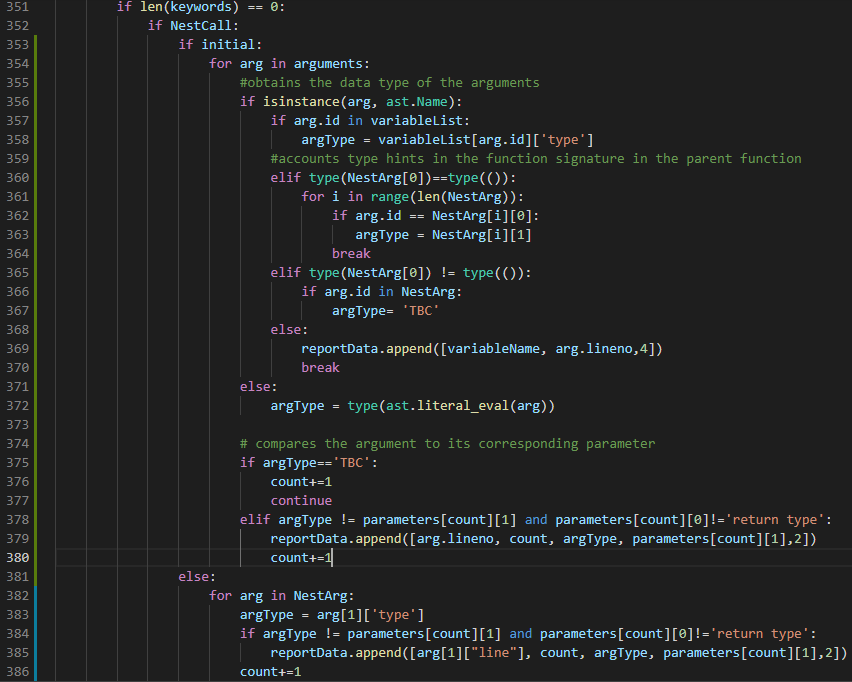
\includegraphics[width=\textwidth, height=12cm]{images/callHintN.png}
    \captionof{figure}{A code snippet of \textbf{callHints} that type checks the consistency of nested method call inputs without keywords.}
    \label{fig:callHintN}
\end{center}

\clearpage
\section{Output/ Report}
Throughout the analysis of a source code, whenever a type error is flagged, an new entry is added to the \textit{reportData} variable. This variable is a collection of all errors identified during the analysis and is categorised by nine different errors, this is detailed in Table \ref{tab:error}.

\begin{table}[H]
\begin{tabular}{|l|l|}
\hline
\textbf{Error type}                                                                                                      & \textbf{Reason for raising the error}                                                                                                                                                   \\ \hline
Data type of variables mismatch                                                                                 & \begin{tabular}[c]{@{}l@{}}When the data type of two variable\\ assignments of the same name mismatch.\end{tabular}                                                            \\ \hline
\begin{tabular}[c]{@{}l@{}}Inconsistency of function inputs with\\ keywords\end{tabular}                        & \begin{tabular}[c]{@{}l@{}}When there is an inconsistency between \\ data types of keywords made in the \\ arguments and the parameter.\end{tabular}                           \\ \hline
\begin{tabular}[c]{@{}l@{}}Inconsistency of function inputs without \\ keywords\end{tabular}                    & \begin{tabular}[c]{@{}l@{}}When there is an inconsistency between \\ data types in the argument with respect\\ to the position in the function signature.\end{tabular}         \\ \hline
Uninitialized variables                                                                                         & \begin{tabular}[c]{@{}l@{}}When the assignment uses an initialized\\ variable.\end{tabular}                                                                                    \\ \hline
\begin{tabular}[c]{@{}l@{}}Mismatch between components of a\\ binary operation\end{tabular}                     & \begin{tabular}[c]{@{}l@{}}When the binary operation contains \\ different data types for its components,\\ maybe unsupported and is generally\\ not recommended.\end{tabular} \\ \hline
\begin{tabular}[c]{@{}l@{}}Mismatch between components of a\\ binary operation in the return value\end{tabular} & \begin{tabular}[c]{@{}l@{}}When the binary operation occurs in the\\ return statement of a function and \\ contains different data types for its\\ components.\end{tabular}    \\ \hline
Undefined function                                                                                              & \begin{tabular}[c]{@{}l@{}}When the function call, calls an undefined\\ function/ class object or is a built-in \\ function outwith the pre-loaded list.\end{tabular}          \\ \hline
Binary operations regarding strings                                                                             & \begin{tabular}[c]{@{}l@{}}When an operand other than add is used\\ for string components.\end{tabular}                                                                        \\ \hline
Uninitialized variable for the return value                                                                     & \begin{tabular}[c]{@{}l@{}}When an initialized variable is used as\\ the return value of a function\end{tabular}                                                               \\ \hline
\end{tabular}
\\
\caption{Table of all possible error types the static analyser detects and the condition to trigger such error}
\label{tab:error}
\end{table}

Once the analysis of a program is complete, the static analyser would print to console:

\begin{itemize}
    \item the local variables defined when functions are defined 
    \item the function signatures defined
    \item the class defined and its associated functions
    \item the global variables initialized
    \item the attributes of objects that has been defined
    \item the errors encountered
    \item the time taken for the analyser to execute
\end{itemize}

All those print statements have an \textit{if} condition that only prints the data when they are applicable to the source code, in other words when the variable that stores those data is not empty with the exception of global variables and the execution time. This was done to reduce the cluttering of the console with unnecessary print statements.



%==================================================================================================================================
\chapter{Evaluation} 
\section{Overview}
The general idea of evaluating the system is by providing the system with multiply different modules for the system to analyse. From there, the outputs will be examined, and a trend graph would be produced to gauge the performance of the system. Afterwards, the modules would also be tested against other \emph{Python} static analysers and its results will be used to validate against the systems output to evaluate its performance to products that are currently used in the market. Figure \ref{fig:eva} shows a flow diagram to visualise this process.

\begin{center}
    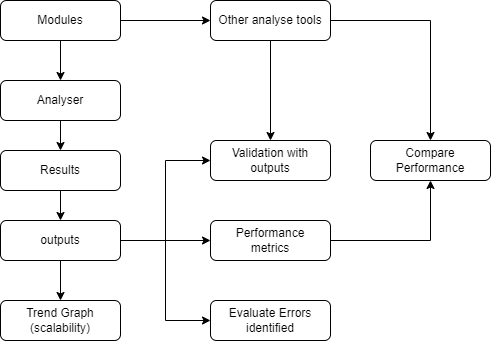
\includegraphics[width=\textwidth]{images/Evalu_flow.png}
    \captionof{figure}{A flow diagram displaying the general process of evaluation}
    \label{fig:eva}
\end{center}

\clearpage
\section{Test Modules}
Each module created is deficient in certain type safe rules and varies in code size allowing different aspects of the analyser to be examined. 

These modules were:
\begin{itemize}
    \item assign\textunderscore test.py
    \item withTH.py
    \item withoutTH.py
    \item function\textunderscore test.py
    \item object\textunderscore test.py
    \item NoTypeHints.py
    \item TypeHints.py
    \item big\textunderscore test.py
\end{itemize}

\textbf{assign\textunderscore test.py} consists of many variable assignments ranging from simple "string" assignments, to subscript (the value in a sequence structure indicated by an index) assignments and assignments of binary operations. As the module contains several type faults such as inconsistency between variable data types, unsupported binary operands and uninitialised variables assignments. The goal of the analyser it to be able to correctly identify these variable assignments and ensure that all the other assignments adhere to the type check rules defined while reporting the ones that do not. The other purpose is to gauge whether the console output correctly filters irrelevant data as the module only consists of variable assignments. The expected output of the analyser would be a list of the global variables defined in the module and identifying the seven errors that are deemed as type faults according to the type safe rules defined.


\textbf{withTH.py}, \textbf{withoutTH.py} and \textbf{function\textunderscore test.py} consists of mainly function definitions and variable assignment function calls to them using a variety of keywords and arguments some which are not recommended or straight up an invalid call. These modules are nearly identical code wise with the exception of \textbf{withTH.py} utilising type hints in all of their function definitions, \textbf{withoutTH.py} utilising none and \textbf{function\textunderscore test.py} implementing type hints on only a few. By using these modules, the performance of the analyser on functions can be observed and determine whether the presence of type hints affects this. The expected output is, most errors found are consistent between the modules and distinct ones are due to the presence of type hints. 

\textbf{object\textunderscore test.py} contains two class definitions, one with methods that do not use type hints while the other one does. The module tests whether the previous mentioned errors above are also applicable to objects and if the analyser is able to identify type errors that are unique to class definitions, ie object method calls out of scope. The expectation of the system is that it will be able to identify these errors but would also have a slightly slower performance relative to its code base size.

To test the scalability of the analyser \textbf{big\textunderscore test.py}, \textbf{NoTypeHints.py}, \textbf{TypeHints.py} were created. These modules are a combination of the other modules with some additional non type safe code to create a variety of code base sizes to gauge the performance of the analyser on larger modules. By doing this, the analyser is able to perform its analysis on more realistic \emph{Python} scripts as these generated scripts contains a mix of everything. The expectation of the outputs are, errors found are consistent with the other errors in their respective modules and that \textbf{big\textunderscore test.py} would have the slowest performance with the other two performing similarly. 

\clearpage
\section{Results}
All results of the static analyser for each module can be found in section \ref{sec:appendix}(Appendices), these include the output of the analyser of the modules and the performance of each tabulated.  

\subsection{assign\textunderscore test.py}
The results from using the analyser on the\textbf{assign\textunderscore test.py} module were seven different statements of the code were deemed not type safe. These errors raised correlates more of the simpler side of type checking which includes: variable consistency, mismatch between components of binary operations, binary operations regarding strings and uninitialized variables as these are more noticeable during development of software.

From the global variables list printed to the console, it can be observed that variables fail to perform a type safe assignment are appointed with the \textit{None} data type. However, if the reason for failure is due to inconsistency in data types between the same variables, then the data type of the earlier assignment is reserved.

\subsection{Function tests}
Using \textbf{withTH.py}, the analyser was able to perform the simple type checks such as consistency data types between variables, made within a function definition, to more complex error checking like validating method calls. In total eight error were flagged for the module and can be seen in Figure \ref{fig:withTH}

From \textbf{withoutTH.py}, five errors were identified. Some which are identical to errors found in \textbf{withTH.py}, for example the inconsistent data type of the "dummy" variable assignment made in the \textit{extend} function, or the uninitialised variable found in the argument of the method call to \textit{check}. Others were due to incapability of arguments and their expected usage within the function. This is because local variables defined in the initial function definition that contains components of the parameter have no data type associated with them hence the analyser bypasses them. However, when method calls are initiated, the data type of the arguments are used for such variables and the whole function is then reevaluated resulting in different outputs dependant of the arguments data type. This shows that without type hints, function are more flexible with their parameters as long as data types of the arguments are compatible with the expected usage. This is evident for the method call of \textit{extend}. In \textbf{withTH.py}, the type hints specify that the parameters must be of data type list hence when the second method call of \textit{extend} occurs, an error is raised as it has integers for its arguments. However, for \textbf{withoutTH.py}, both method calls pass the type check analysis as they are both compatible with the expected usage. Another difference between the two modules are, since in \textbf{withoutTH.py} variables are bypassed of type checking during the initial function definition due to unknown data types of variables, the data type of such variables when printed to console is just a reference to the node that assignment variable. Whereas, for \textbf{withTH.py} all data types are known thus all references to functions, their data types are all specified. 

Since \textbf{function\textunderscore test.py} is a combination of functions with/out type hints, the analysis also corresponds this. As in, the errors found are nearly identical to the ones encountered in \textbf{withoutTH.py} and \textbf{withTH.py} and functions without type hints also inherits the property of referencing nodes for its local variables and function signatures.

\begin{center}
    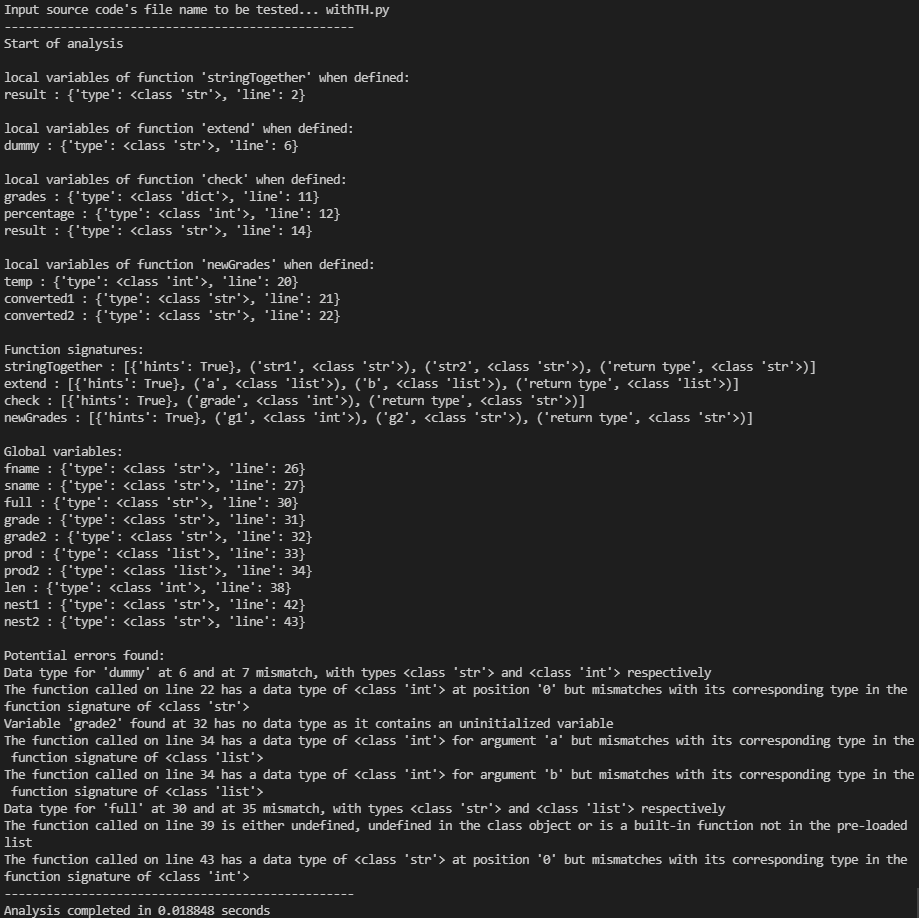
\includegraphics[width=\textwidth]{images/withTH.png}
    \captionof{figure}{A screenshot of the output of the analysis of \textbf{withTH.py} produced by the static analyser}
    \label{fig:withTH}
\end{center}

\subsection{object\textunderscore test.py}
The static analyser was able to successfully perform analysis on class objects. This is evident through analysing the \textbf{object\textunderscore test.py} module. The analyser was able to track, type check and update attributes were applicable. This is shown with attribute "grade" found in the class object of \textit{student}. It is first initiated in the \textit{saveGrade} method where type hints are not defined, hence the attribute, "grade", can be of any type. Afterwards, the same method call is used but with a different argument and type which results in an inconsistent variable data type error. This also implies that the validity of data types in method call also works for class objects. An error unique to class objects is the use of method calls outwith the class (out of scope). For example, the variable "compsci" is an instance of the class\textit{course} and only has the functions: \textit{init}, \textit{capacity}, \textit{coordinator} and \textit{AvgGrade}. So when the module tries to perform the method of \textit{getYear} in the \textit{compsci} instance it will result in an undefined method call error. Overall the analyser highlighted five code statements as not type safe.

\subsection{Big Modules}
As mentioned before, \textbf{big\textunderscore test.py}, \textbf{NoTypeHints.py} and \textbf{TypeHints.py} modules are a combination of the other modules with some additional code so the output of the analysis are significantly long than the others. It can be concluded regardless of the size of the source code, the analyser is consistent with its outputs as the analyser was able to identify the same errors found in the other modules while also identifying new errors produced by the additional code.

\subsection{Performance/ scalablitiy}
Each module was analysed five times to calculate the average of the execution time for the static analyser to complete, Table \ref{tab:exe}. This was to obtain a more accurate representation of the performance. By doing this, the consistency rate can also be gauged increasing the reliability of the analysis of the program.

\begin{table}[h]
\centering
\begin{tabular}{|l|c|}
\hline
Module            & Average execution time (ms) \\ \hline
assign\_test.py   & 12.4996                  \\ \hline
withTH.py         & 16.5686                  \\ \hline
withoutTH.py      & 18.1082                  \\ \hline
function\_test.py & 16.8592                  \\ \hline
object\_test.py   & 23.9076                  \\ \hline
NoTypeHints.py    & 37.3184                  \\ \hline
TypeHints.py      & 38.1918                  \\ \hline
big\_test.py      & 45.7308                  \\ \hline
\end{tabular}
    \caption{The average execution times for the static analyser to perform its analysis on modules}
\label{tab:exe}
\end{table}

From the Table \ref{tab:exe}, it can be observed that \textbf{assign\textunderscore test.py} has the fastest execution time which is due the simplicity of the module containing only variable assignments thus not many type checks rules defined applies. Following that is the function tests with \textbf{withTH.py} performing quickest followed by \textbf{function\textunderscore test.py} and \textbf{withoutTH.py}. This is within reason as with type hints, function signatures all know their types so it is only a matter of obtaining the data types and comparing them to ensure they are valid method calls. Whereas, without type hints, data types needs to be acquired through the arguments, saved into a new variable and traverse the function definition node a second time to ensure it is type safe, hence the increase in execution time. And since \textbf{function\textunderscore test.py} is a combination of both it is logical that it is in the middle. \textbf{object\textunderscore test.py} performs slower than the function tests as in addition to containing functions with/out type hints, the analyser also needs to perform an extra set of iterations to locate the class object before the functions. The larger modules of \textbf{NoTypeHints.py} and textbf{TypeHints.py} further supports the argument made on the performance of functions due to the presence of typehints. As although \textbf{TypeHints.py} is a larger module than \textbf{NoTypeHints.py} the performance difference is only by a fraction of a millisecond. As although \textbf{TypeHints.py} is a larger module than \textbf{NoTypeHints.py} the performance difference is only by a fraction of a millisecond. Finally \textbf{big\textunderscore test.py} has the slowest execution time. This is to be expected due to the size of the module compared to the others and since it contains a mix of everything. 

To answer the scalability of the static analyser a scatter graph was created and a line of best fit was determined. The graph used the number of code lines in the module as the independent variables and the execution time as the dependent variable, Figure \ref{fig:graph}. All modules except \textbf{withTH.py} and \textbf{withoutTH.py} were used to create the graph as they all vary in code base size. The modules opted out for the graph were because those and \textbf{function\textunderscore test.py} have the same code base size so the one with median of the three was chosen.

\begin{center}
    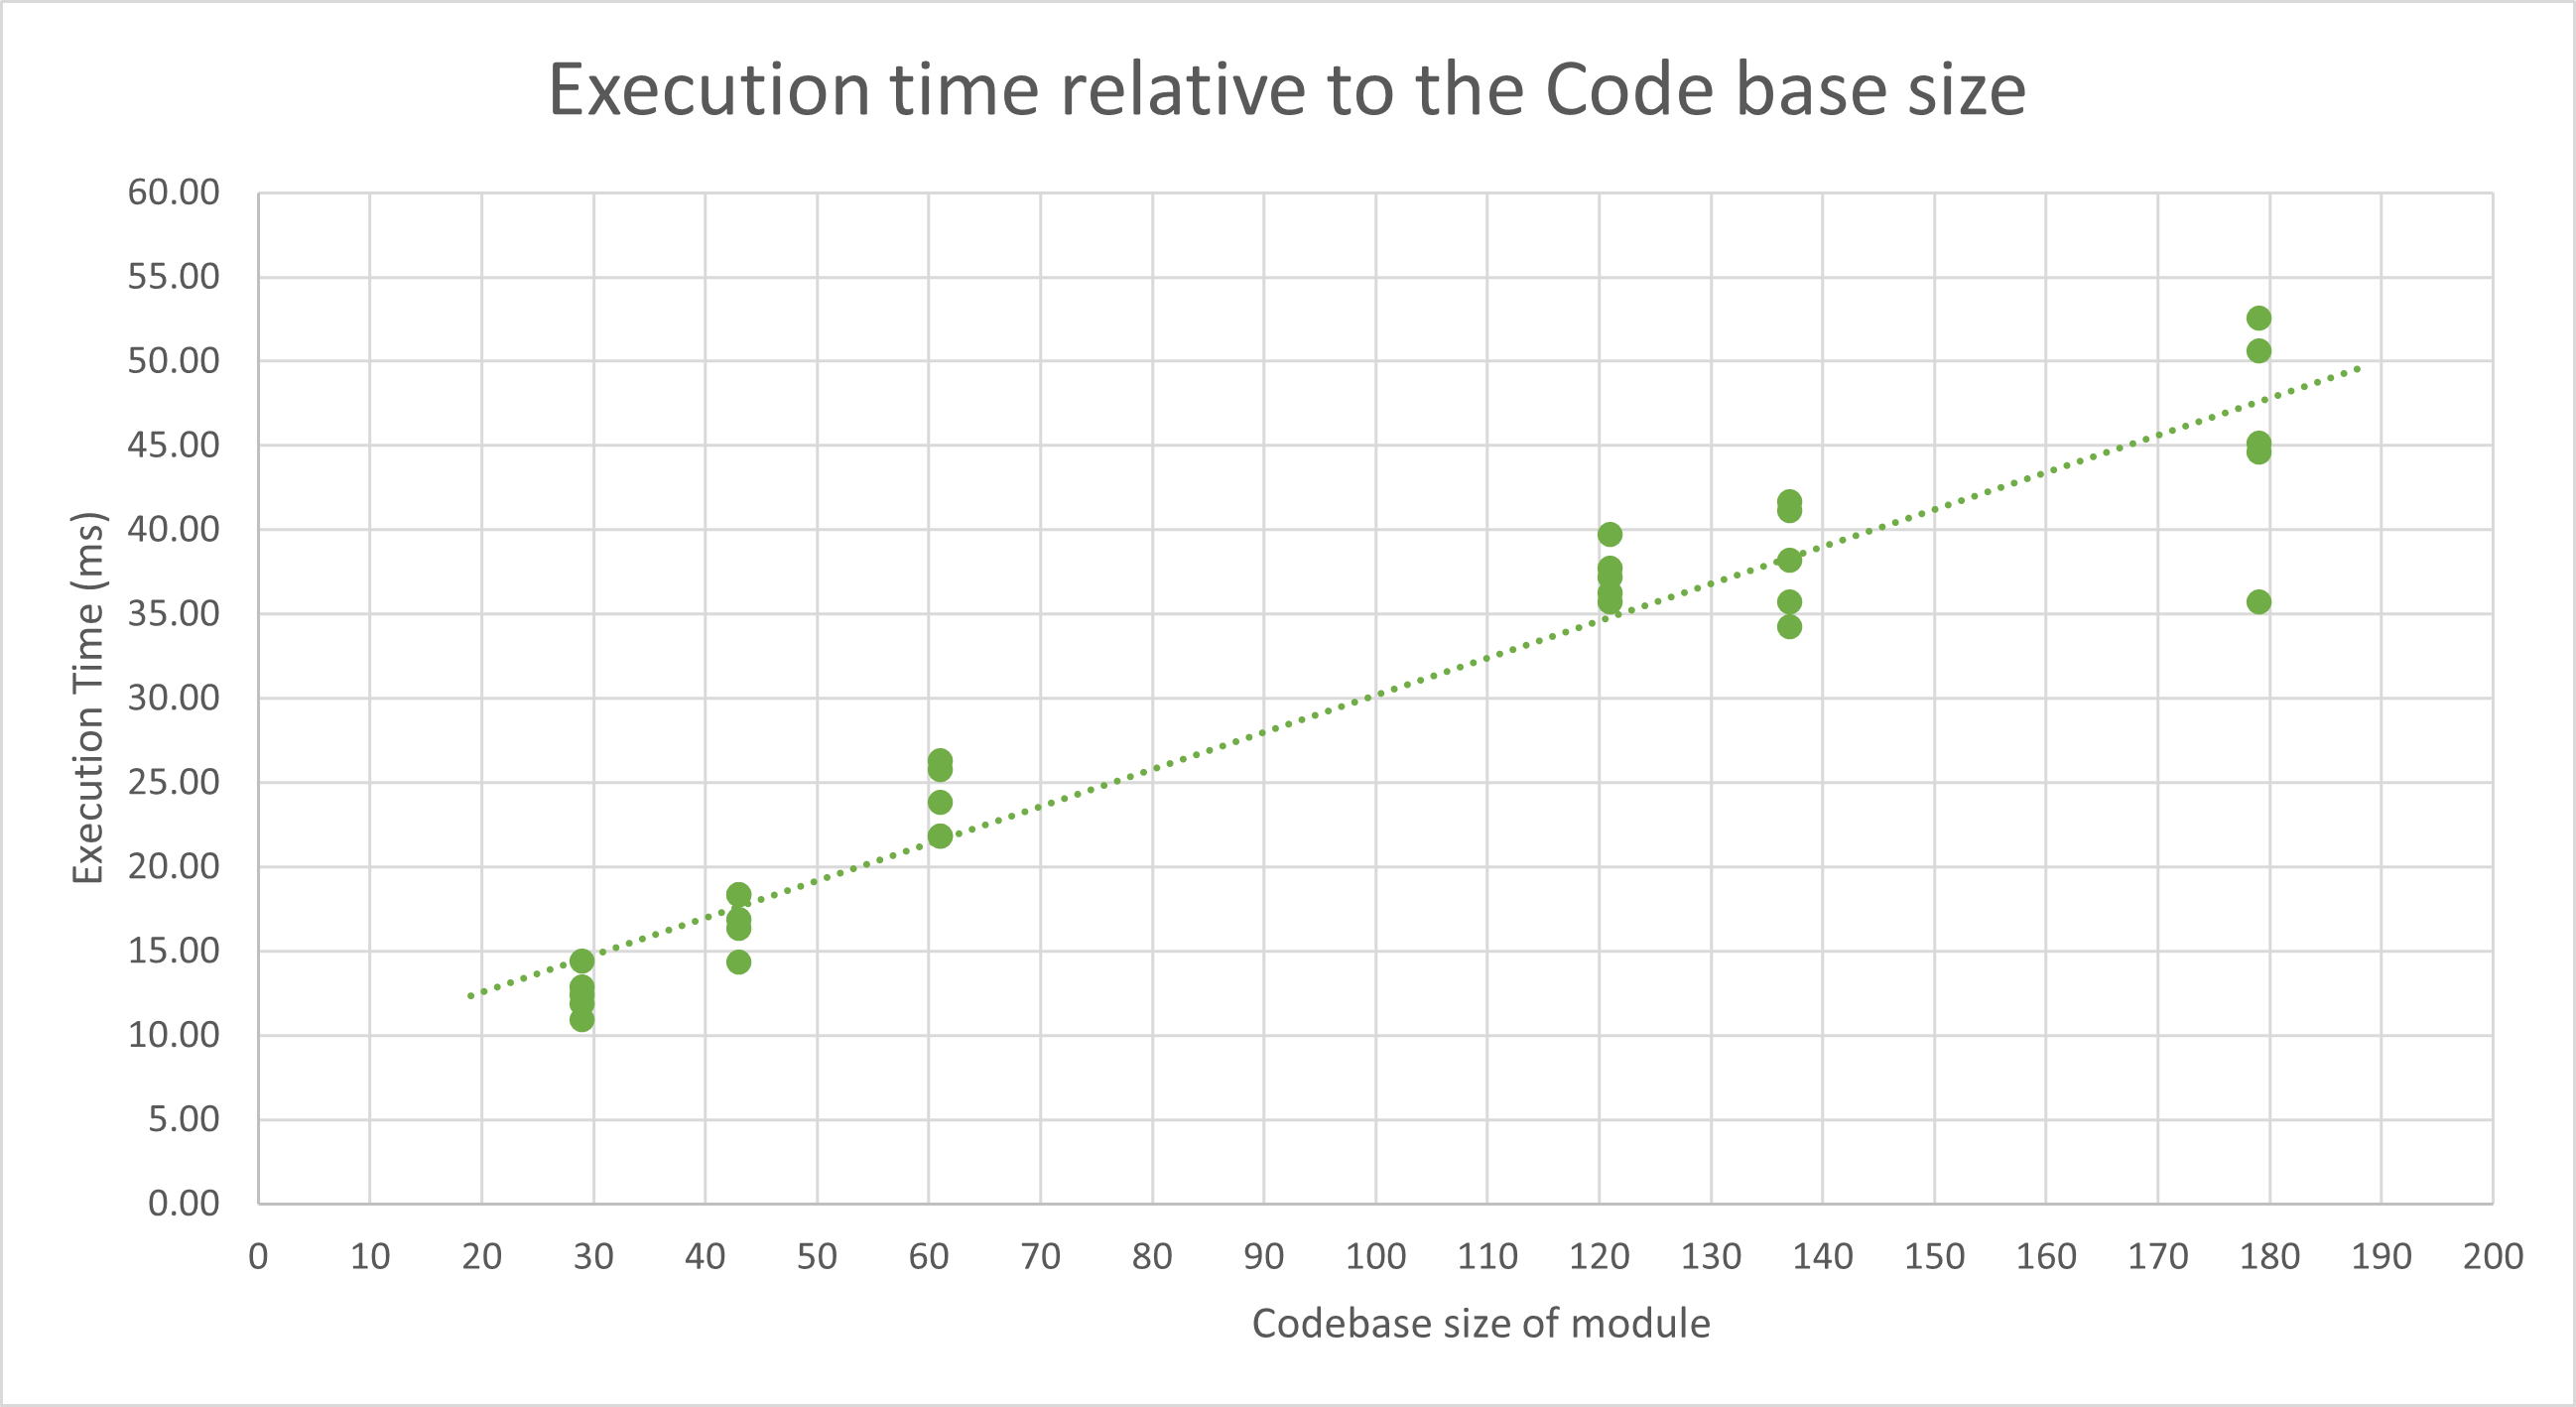
\includegraphics[width=\textwidth]{images/Graph.png}
    \captionof{figure}{A scatter graph with a line of best fit plotted to show the relationship between the execution time and the size of the code base being analysed, data can be found in the Appendix \ref{tab:exe1}}
    \label{fig:graph}
\end{center}

From the Figure \ref{fig:graph}, it can be concluded that the static analyser has a linear relationship between the execution time and the size of code base it analyses. This implies that as the code base of the module increases, the time to perform the analysis also increases in a linear fashion.

\subsection{Validity with mypy}
Since \emph{mypy} is a static analyser that only type checks assignments and functions and classes that use type hints, only few of the modules can be evaluated. 

With the \textbf{assign\textunderscore test.py} module \textit{mypy} reported six errors. All the reported errors correspond to the ones found by the system. However, \textit{mypy} did not flag the Binary operation assignment for "area" made on code line 16 of the module. This is because using the multiplication operand on a list and an integer is supported by \emph{Python}, hence it was not flagged. But this kind operand of different data types could potentially lead to problems for example on a dictionary and a integer, thus as a general rule the system would flag this as an error.

Using the \textit{mypy} analyser on the \textbf{withTH.py} module, a total of nine errors were accumulated. Eight of which matches what the system outputs. The additional one found by \textit{mypy} was on code line 38 and was probably the result of using the same variable name as the function "len" hence it was unable to determine the type. As when the variable name was changed to "length", the associated error was not flagged anymore. 

When using the module \textbf{TypeHints.py}, \textit{mypy} had identified 28 non type safe applications.
Of the identified ones, all were also highlighted by the system. However, the system did report an extra two errors, both are of the same kind. The error was due to the binary operation performing an unsupported operation of two data types, resulting in an error. But that error carried over to the variable assignment consistency type check causing this to report the error that \textit{mypy} did not identify. Essentially, the system reported the same error twice due to how the consistency type check handles \textit{None} types.

Since the \textbf{object\textunderscore test.py} module half uses type hints, ie one class uses them and the other does not, only the one with type hints is type checked by \textit{mypy}. This results in two errors raised which also coincides with the ones reported by the system.

From these results, it can be concluded that the analysis from the system for assignments and type hints is fairly accurate in that it was able to match the errors identified by an static analyser that is widely used by the public. 

In addition to this, by using the shell script command in Listing \ref{lst:shell}, we are able to obtain the execution time of \textit{mypy} for each relevant modules, ie the ones that consist of type hints.

\begin{lstlisting}[caption= The shell script command used to obtain the execution time of mypy where module.py is replaced with the name of the module that is going to be analysed, label={lst:shell}]
Measure-Command{mypy module.py}
\end{lstlisting}

This is then tabulated in Table \ref{tab:mypy} and a scatter plot graph between \textit{mypy} times and the systems times is plotted to assist in visualising the difference.

\begin{table}[h]
\centering
\begin{tabular}{|l|l|l|}
\hline
Module            & Code Size & Time (ms) \\ \hline
assign\_test.py   & 29        & 370.6694  \\ \hline
withTH.py         & 43        & 359.8141  \\ \hline
function\_test.py & 43        & 367.0797  \\ \hline
object\_test.py   & 61        & 366.9547  \\ \hline
TypeHints.py      & 137       & 373.291   \\ \hline
big\_test.py      & 179       & 366.6376  \\ \hline
\end{tabular}
\caption{Table of execution times of mypy}
\label{tab:mypy}
\end{table}

\begin{center}
    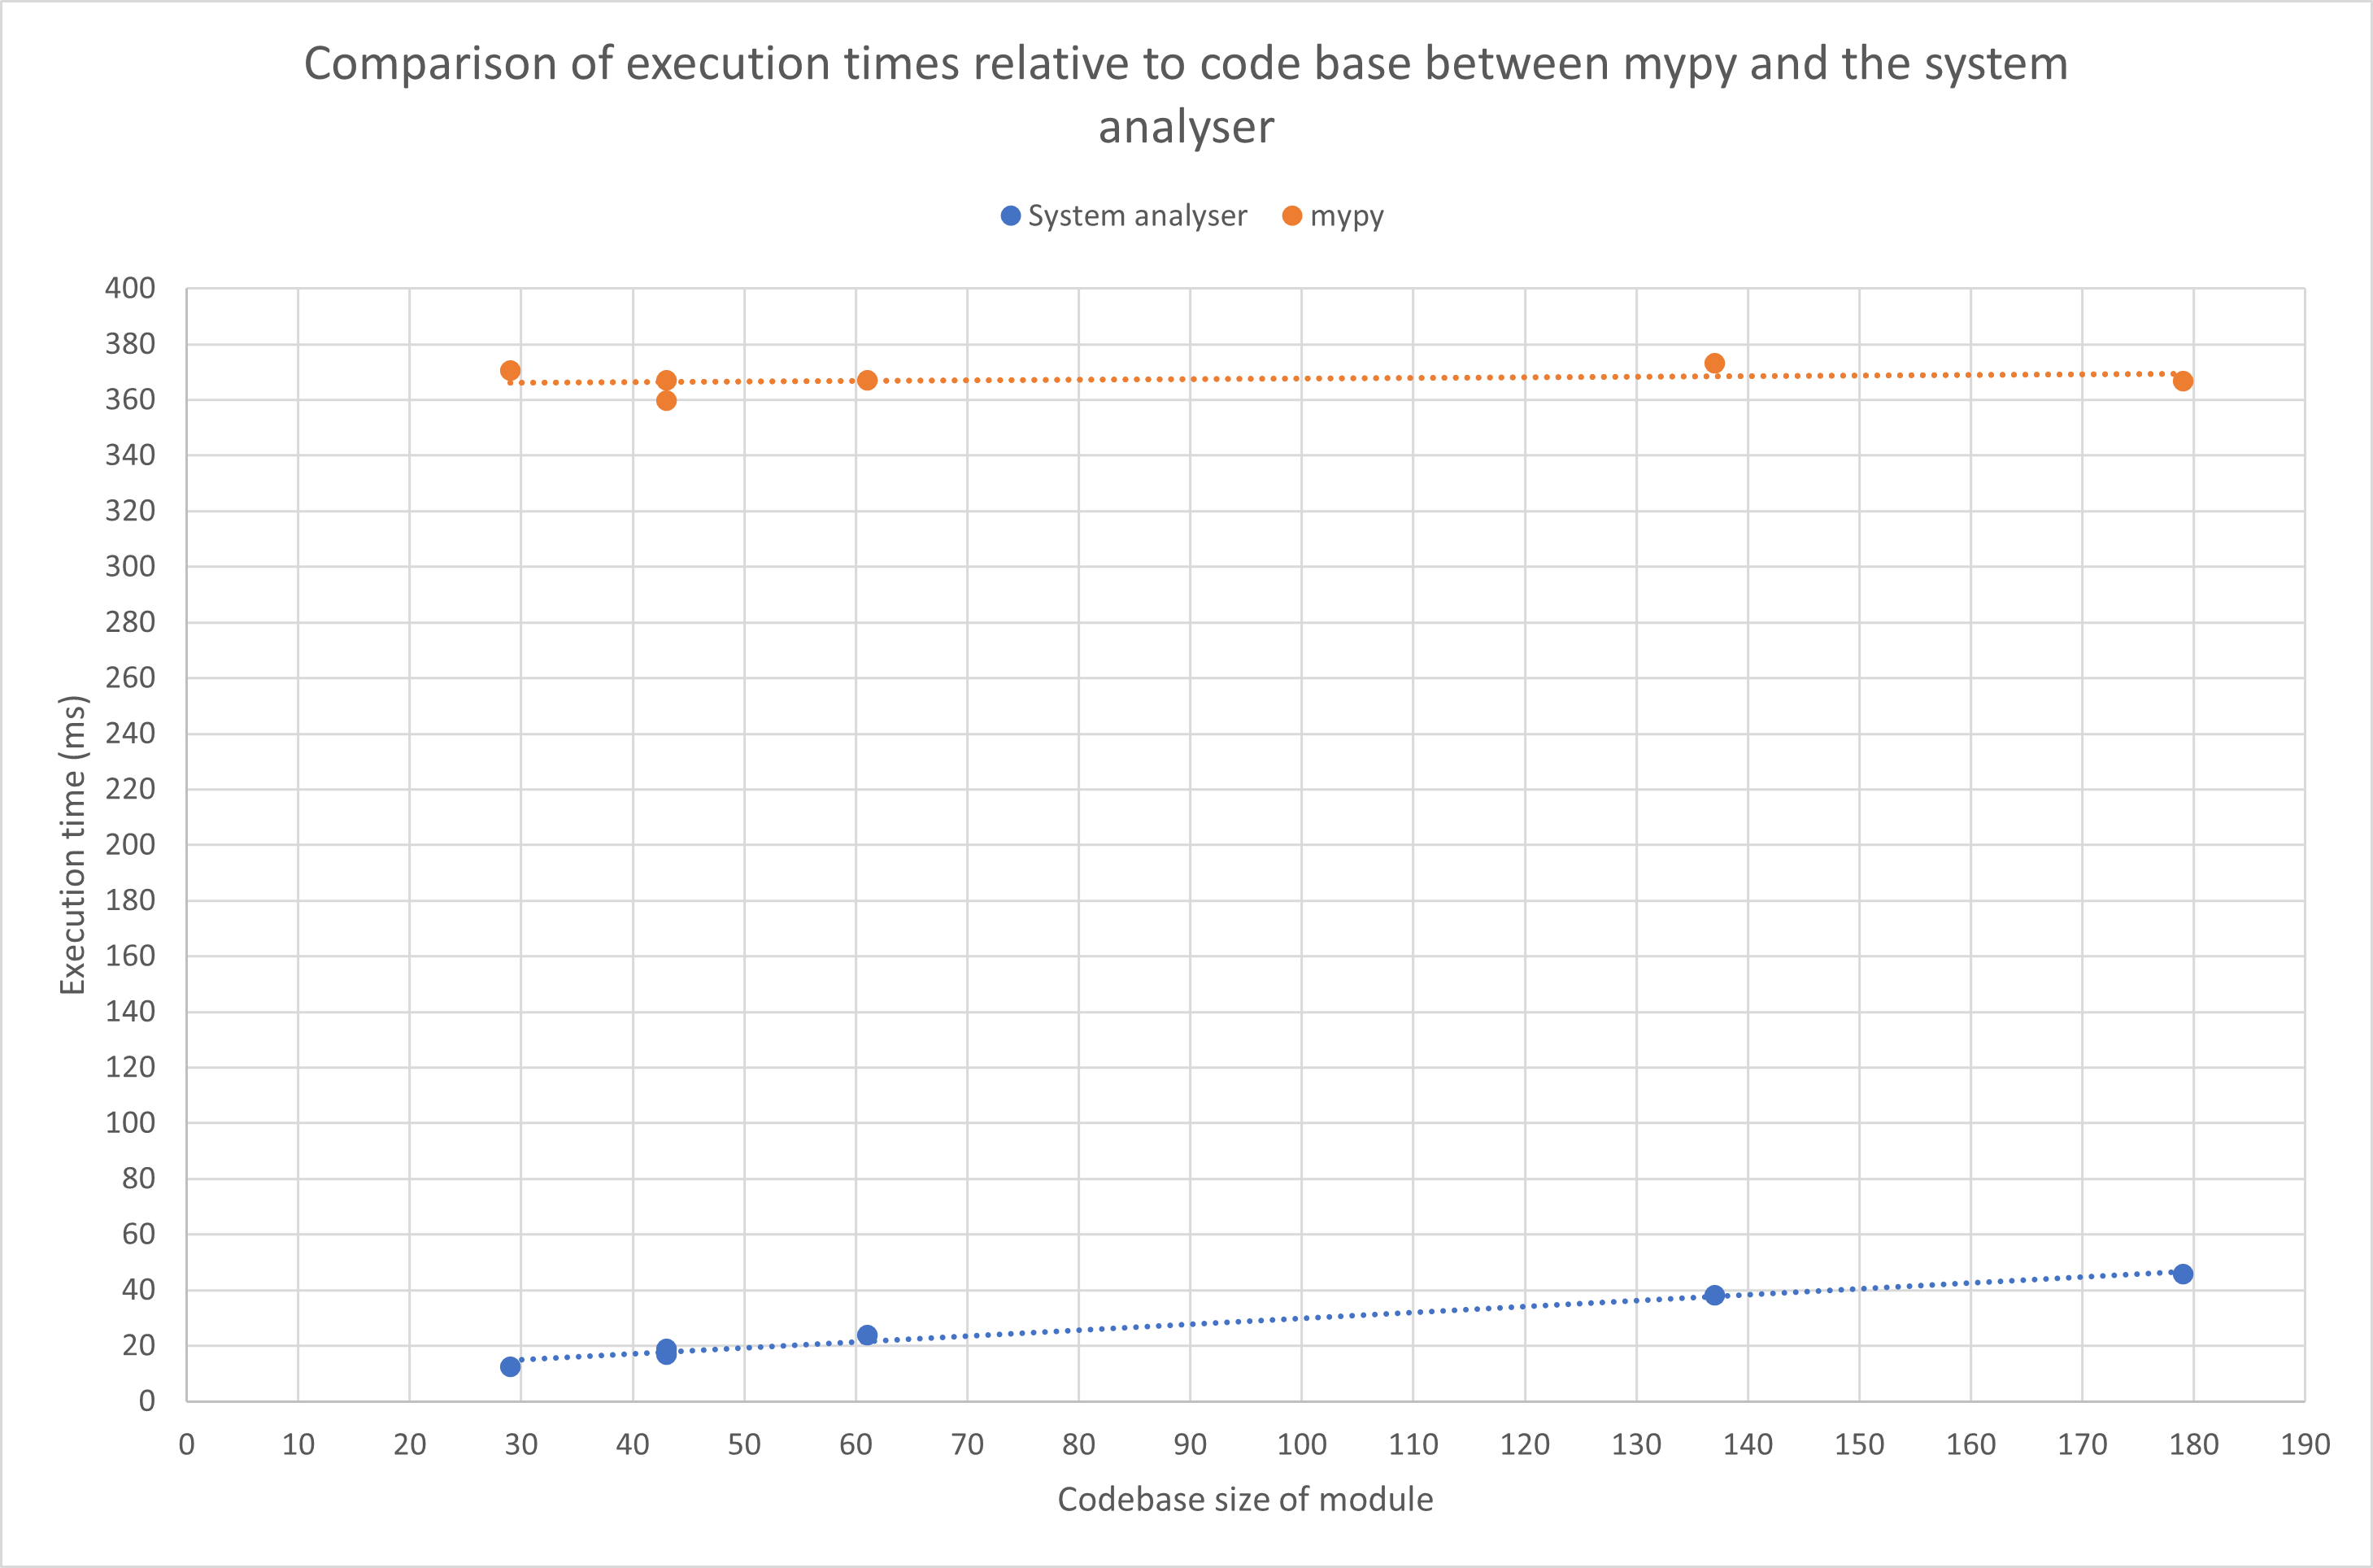
\includegraphics[width=\textwidth]{images/mypyG.png}
    \captionof{figure}{A scatter graph with the line of best fit plotted against each analyser to evaluate the differences, data points can be found in Table \ref{tab:exe} and Table \ref{tab:mypy}}
    \label{fig:graph1}
\end{center}

From Figure \ref{fig:graph1}, it can be observed that mypy's trend line is almost flat implying that regardless of what the code base size it is analysing it will have similar execution times. Whereas, although the system analysis is significantly faster than mypy's at the tested code base size, it has increasing linear trend line. Thus, if the trend line is extrapolated far enough to a \textbf{very} large code base, then performance of the system analyser would gradually decrease and perhaps even perform slower that mypy since its performance is constant. 
%==================================================================================================================================
\chapter{Discussion}    
This chapter discusses some of the sacrifices made in order to implement the program, while also suggesting what other features that could be added to the program if more time was given.

\section{Limitations}
Due the vast amount of data types available within the \emph{Python} language, the program mainly focuses on type checking the most commonly used data types:
\begin{itemize}
    \item Integers
    \item Floating point numbers 
    \item Strings
    \item Boolean
    \item Sequence Types such as List and Tuple
    \item Dictionaries
\end{itemize}

However, as the collection type data structures can contain different data type for their components, the type check performed for these are between the data structures rather than their individual components. This is because the actual values of the data structure is not stored but only the type of the structure. Hence when the components of data structures are called/ used they are assigned the generic type "subscript" rather than their actual data type.

Another limitation set is, only the \emph{Python} built-in and user-defined functions are considered for type checking functions. This is because not all external functions are well documented, thus, obtaining the data types of the in/outputs required of these functions are too complex within the given time frame. 

\section{Future work/ Improvements}

A feature which could improve the performance to the system, is by implementing an ordered data structures like a Binary Search Tree or a sorted list  to store variables rather than non ordered ones. This is because it would increase the speed of searching of variables by only requiring to search through half the data structure. Since when the data structure is ordered, searches can begin from the middle and iterate either left or right depending on if the target is greater than or less then the current value.

Another improvement that could be made is by creating additional test cases, that could be more complex or test the extremities of the system. For example if testing complexity, a much larger code base size say 1000 that contains multiple different components and maybe several recursive/ nested functions could be used. This would increase the completeness of the experiments made and also soundness of the system.

One other future work that could be done to the system is changing the method of obtaining code modules from users. As currently, users can only analyse one code module per analyser execution. So it could be beneficial if the system could, say for example receive a file directory with multiple code modules within, and the system would be able to perform analysis on each in a single execution. With this feature, it would increase the overall productivity of the user and reduce tedious nature of have to run the same execution but for different module multiple times.

%==================================================================================================================================
\chapter{Conclusion}    
\section{Summary}
The project aim was to develop a static analyser that performs an evaluation on code bases provided by the user written in the Dynamically typed language \emph{Python}. The analyser would be able to function in and out with integrated development environments. To achieve this, the analyser had to accomplish the must and should have requirements specified in chapter 3. And from the requirements a design methodology was derived, where an abstract syntax tree is created from a given code base. Afterwards the analyser would iterate through the nodes in the tree visiting, visitor functions that are associated with the node. Then the relevant data in the nodes are extracted and are analysed for type safe and finally a report is produced with the results from the analysis.

Overall, the static analyser developed was successful as it achieved most of the requirements set and the outputs of the analysis were deemed accurate through validating them with the outputs of the widely used static analyser \emph{mypy}. It was also concluded that the system performance scales linearly relative to the size of the code base. Though, there are also limitations of the system due to the flexible nature of \emph{Python}, therefore extra features could be implemented to improve the static analyser.

\section{Reflection}
From working on this project, I have been taught plentifully in terms of individually conducting a large-scaled project. Starting from just a small specification to a full fledged working product. It has proved the significance of being able to properly prioritise the workload to be within the time constraint. The difficulty of designing a variety of test modules suitable for the static analyser while also tailoring them to produce certain errors was also made clear. If I was to do the project differently, I would definitely research more about the techniques utilized by other \emph{Python} type checkers and what sort of data structures they used.
%==================================================================================================================================
%
% 
%==================================================================================================================================
%  APPENDICES  

\begin{appendices}

\chapter{Appendices}
\label{sec:appendix}
\section{Analyser outputs}
\begin{center}
    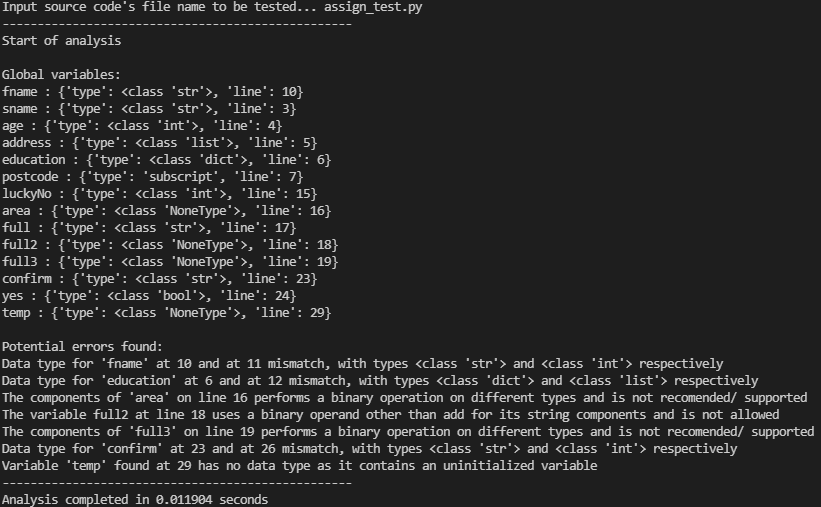
\includegraphics[width=\textwidth]{images/assign.png}
    \captionof{figure}{A screenshot of the output of the analysis of \textbf{assign\textunderscore test.py} produced by the static analyser}
\end{center}

\begin{center}
    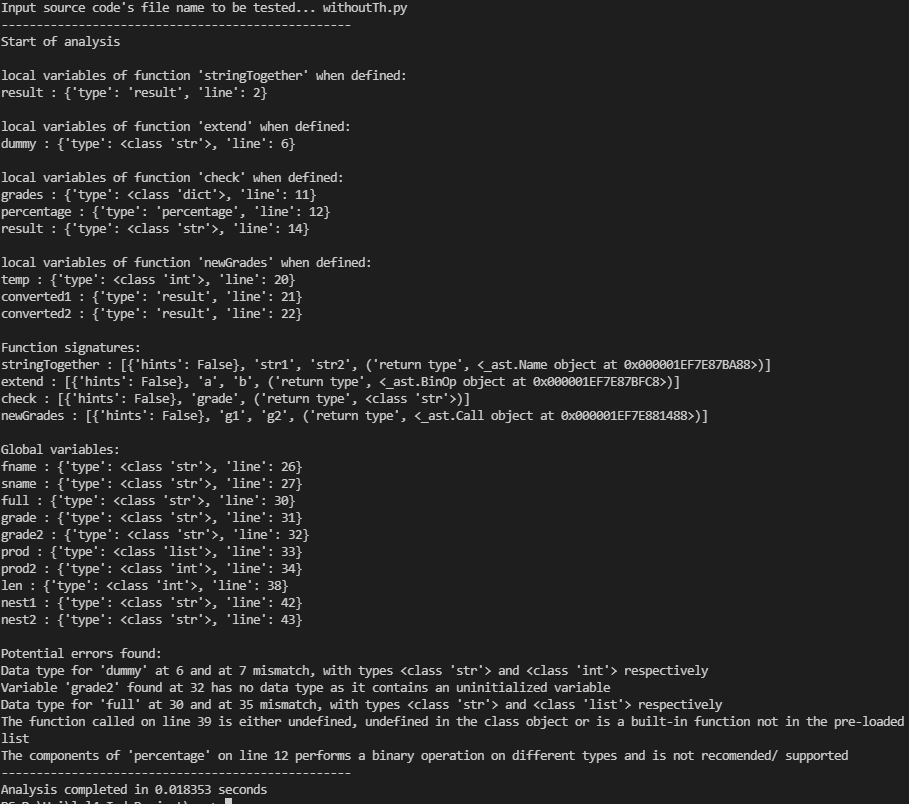
\includegraphics[width=\textwidth]{images/withoutTH.png}
    \captionof{figure}{A screenshot of the output of the analysis of \textbf{withoutTH.py} produced by the static analyser}
\end{center}

\begin{center}
    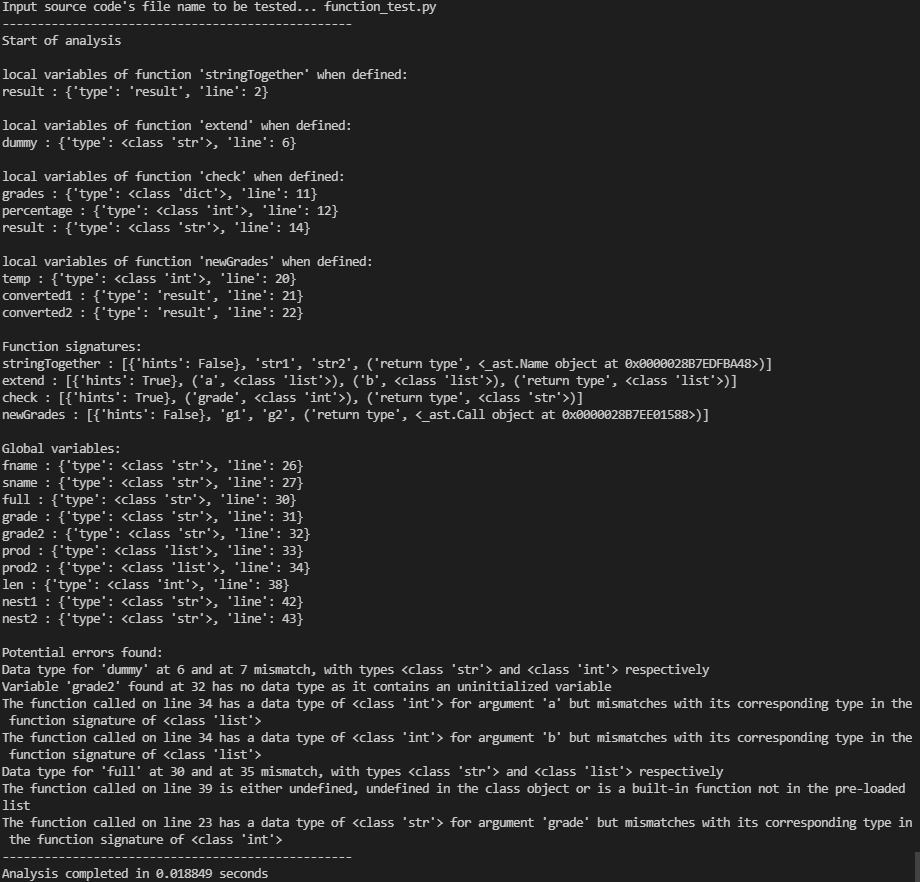
\includegraphics[width=\textwidth]{images/function_test.png}
    \captionof{figure}{A screenshot of the output of the analysis of \textbf{function\textunderscore test.py} produced by the static analyser}
\end{center}

\begin{center}
    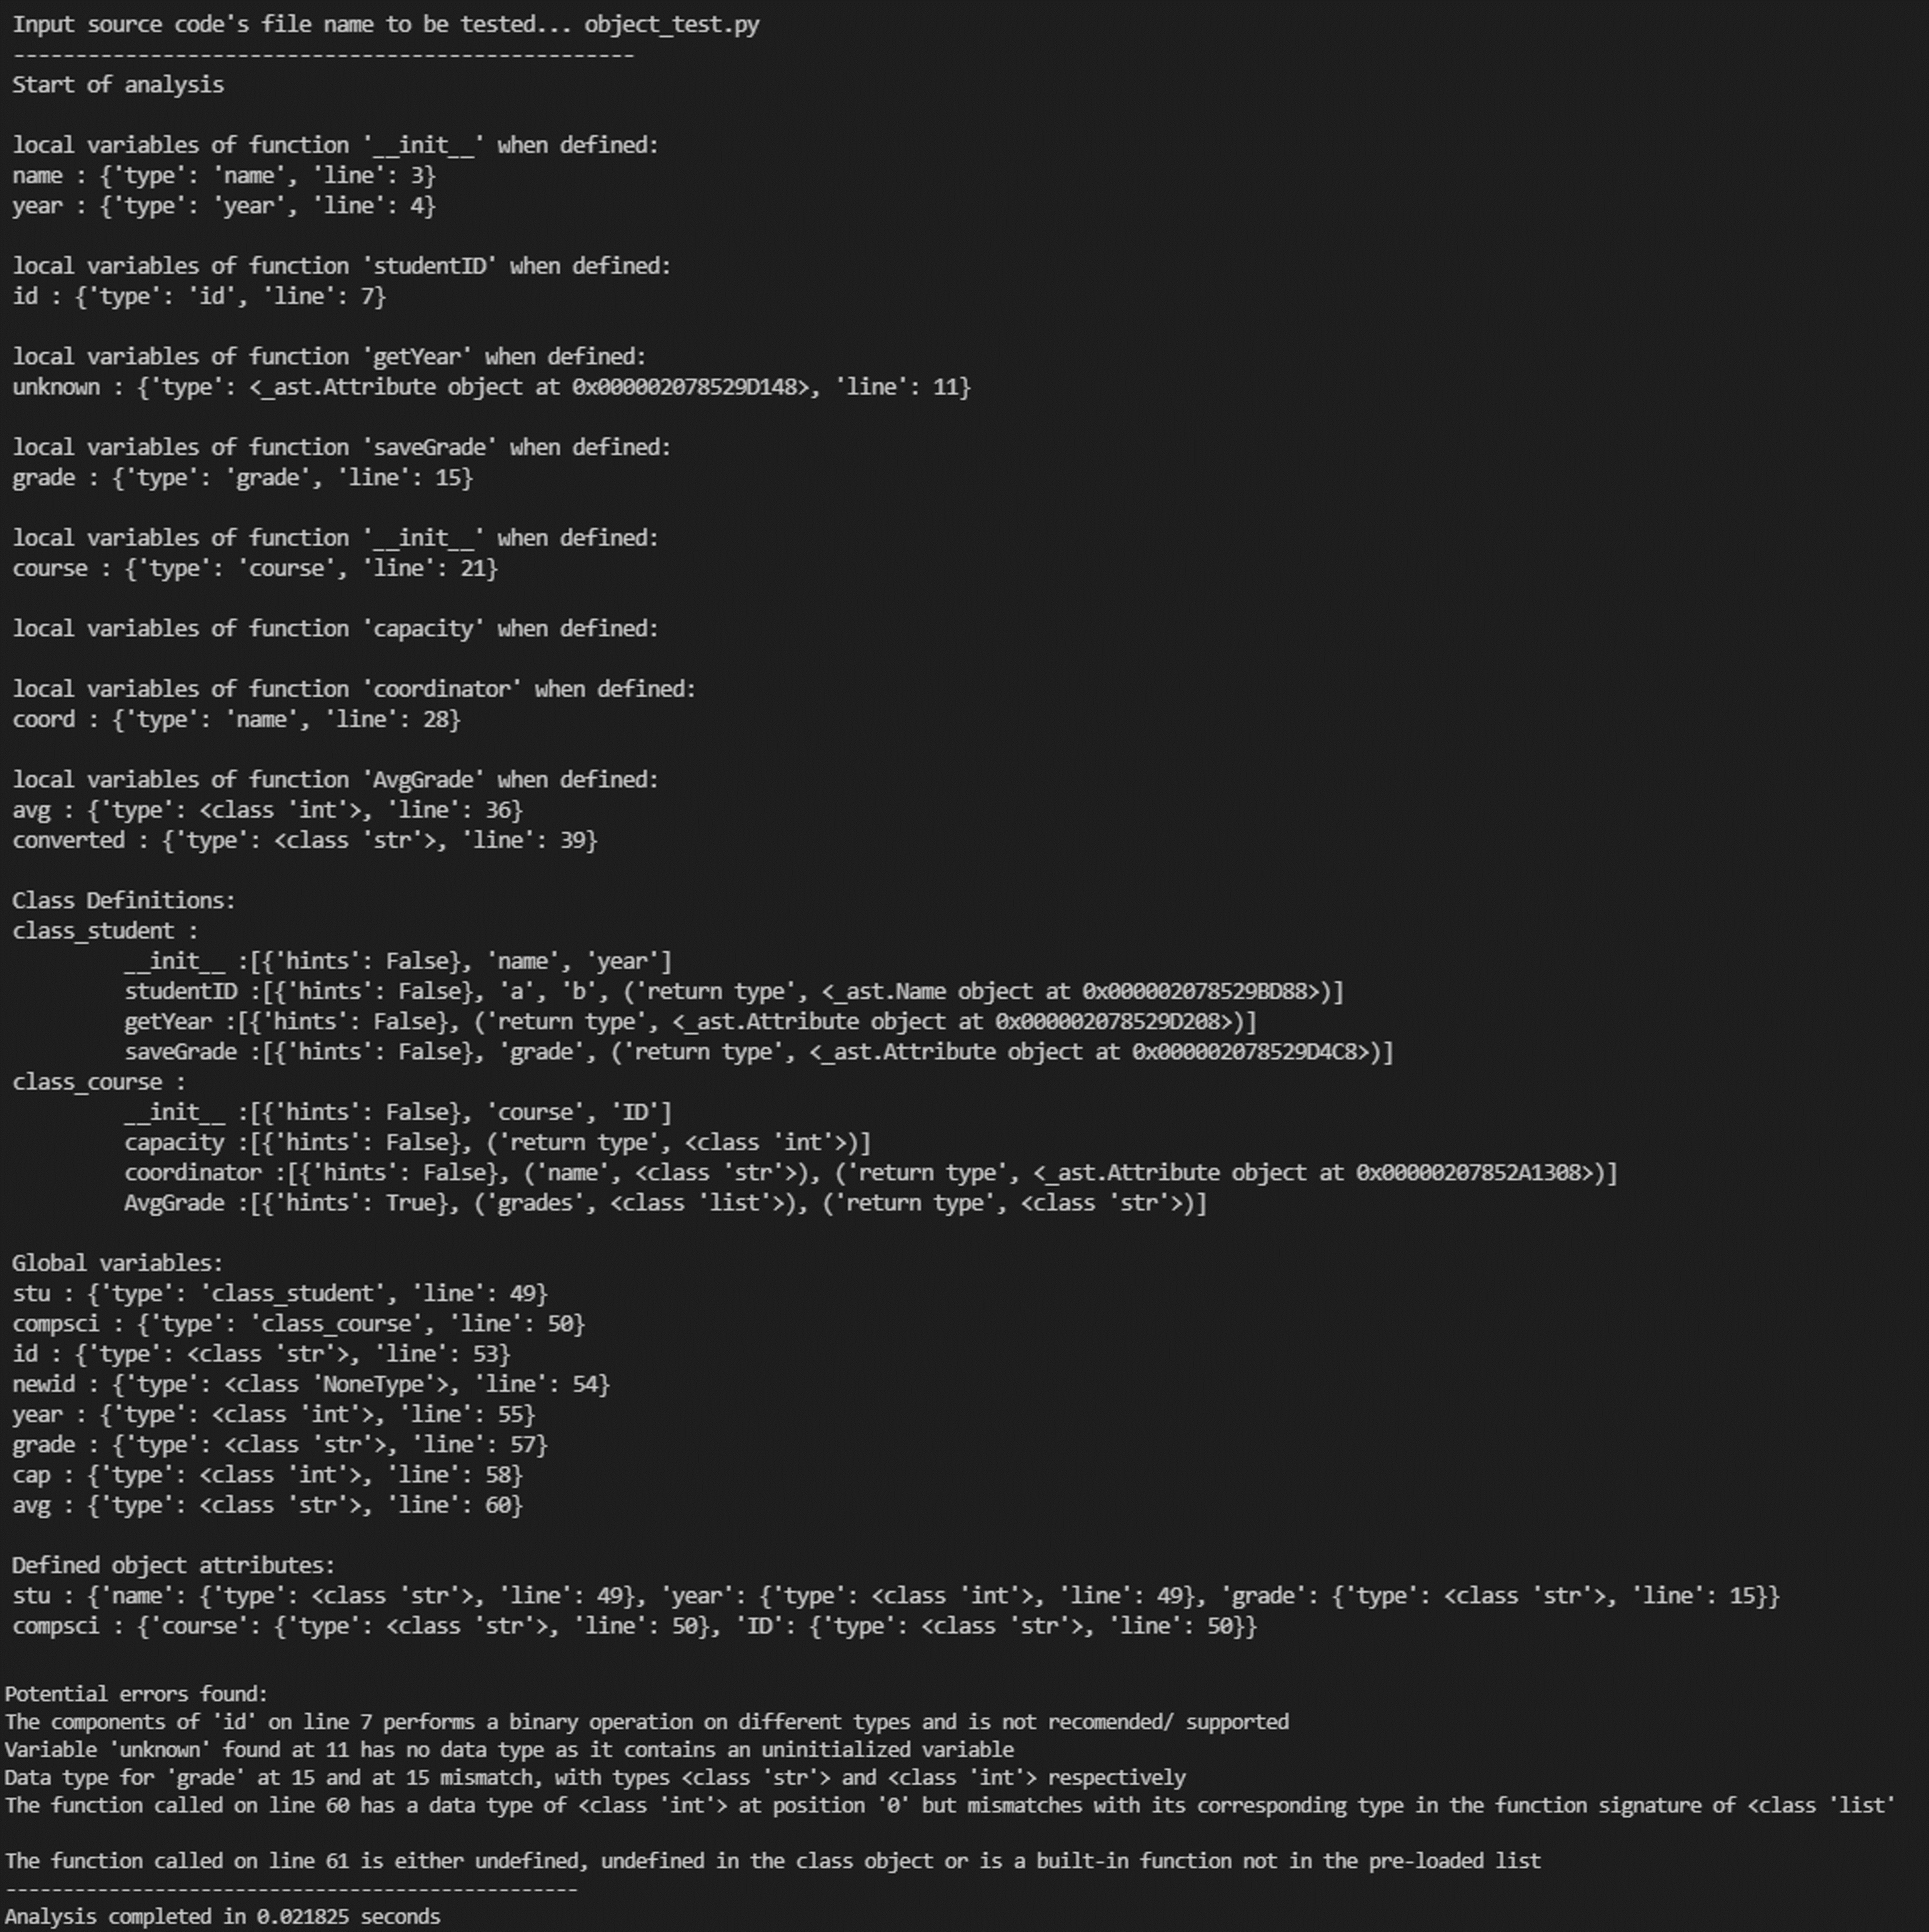
\includegraphics[width=\textwidth]{images/object_test.png}
    \captionof{figure}{A screenshot of the output of the analysis of \textbf{object\textunderscore test.py} produced by the static analyser}
\end{center}

\begin{center}
    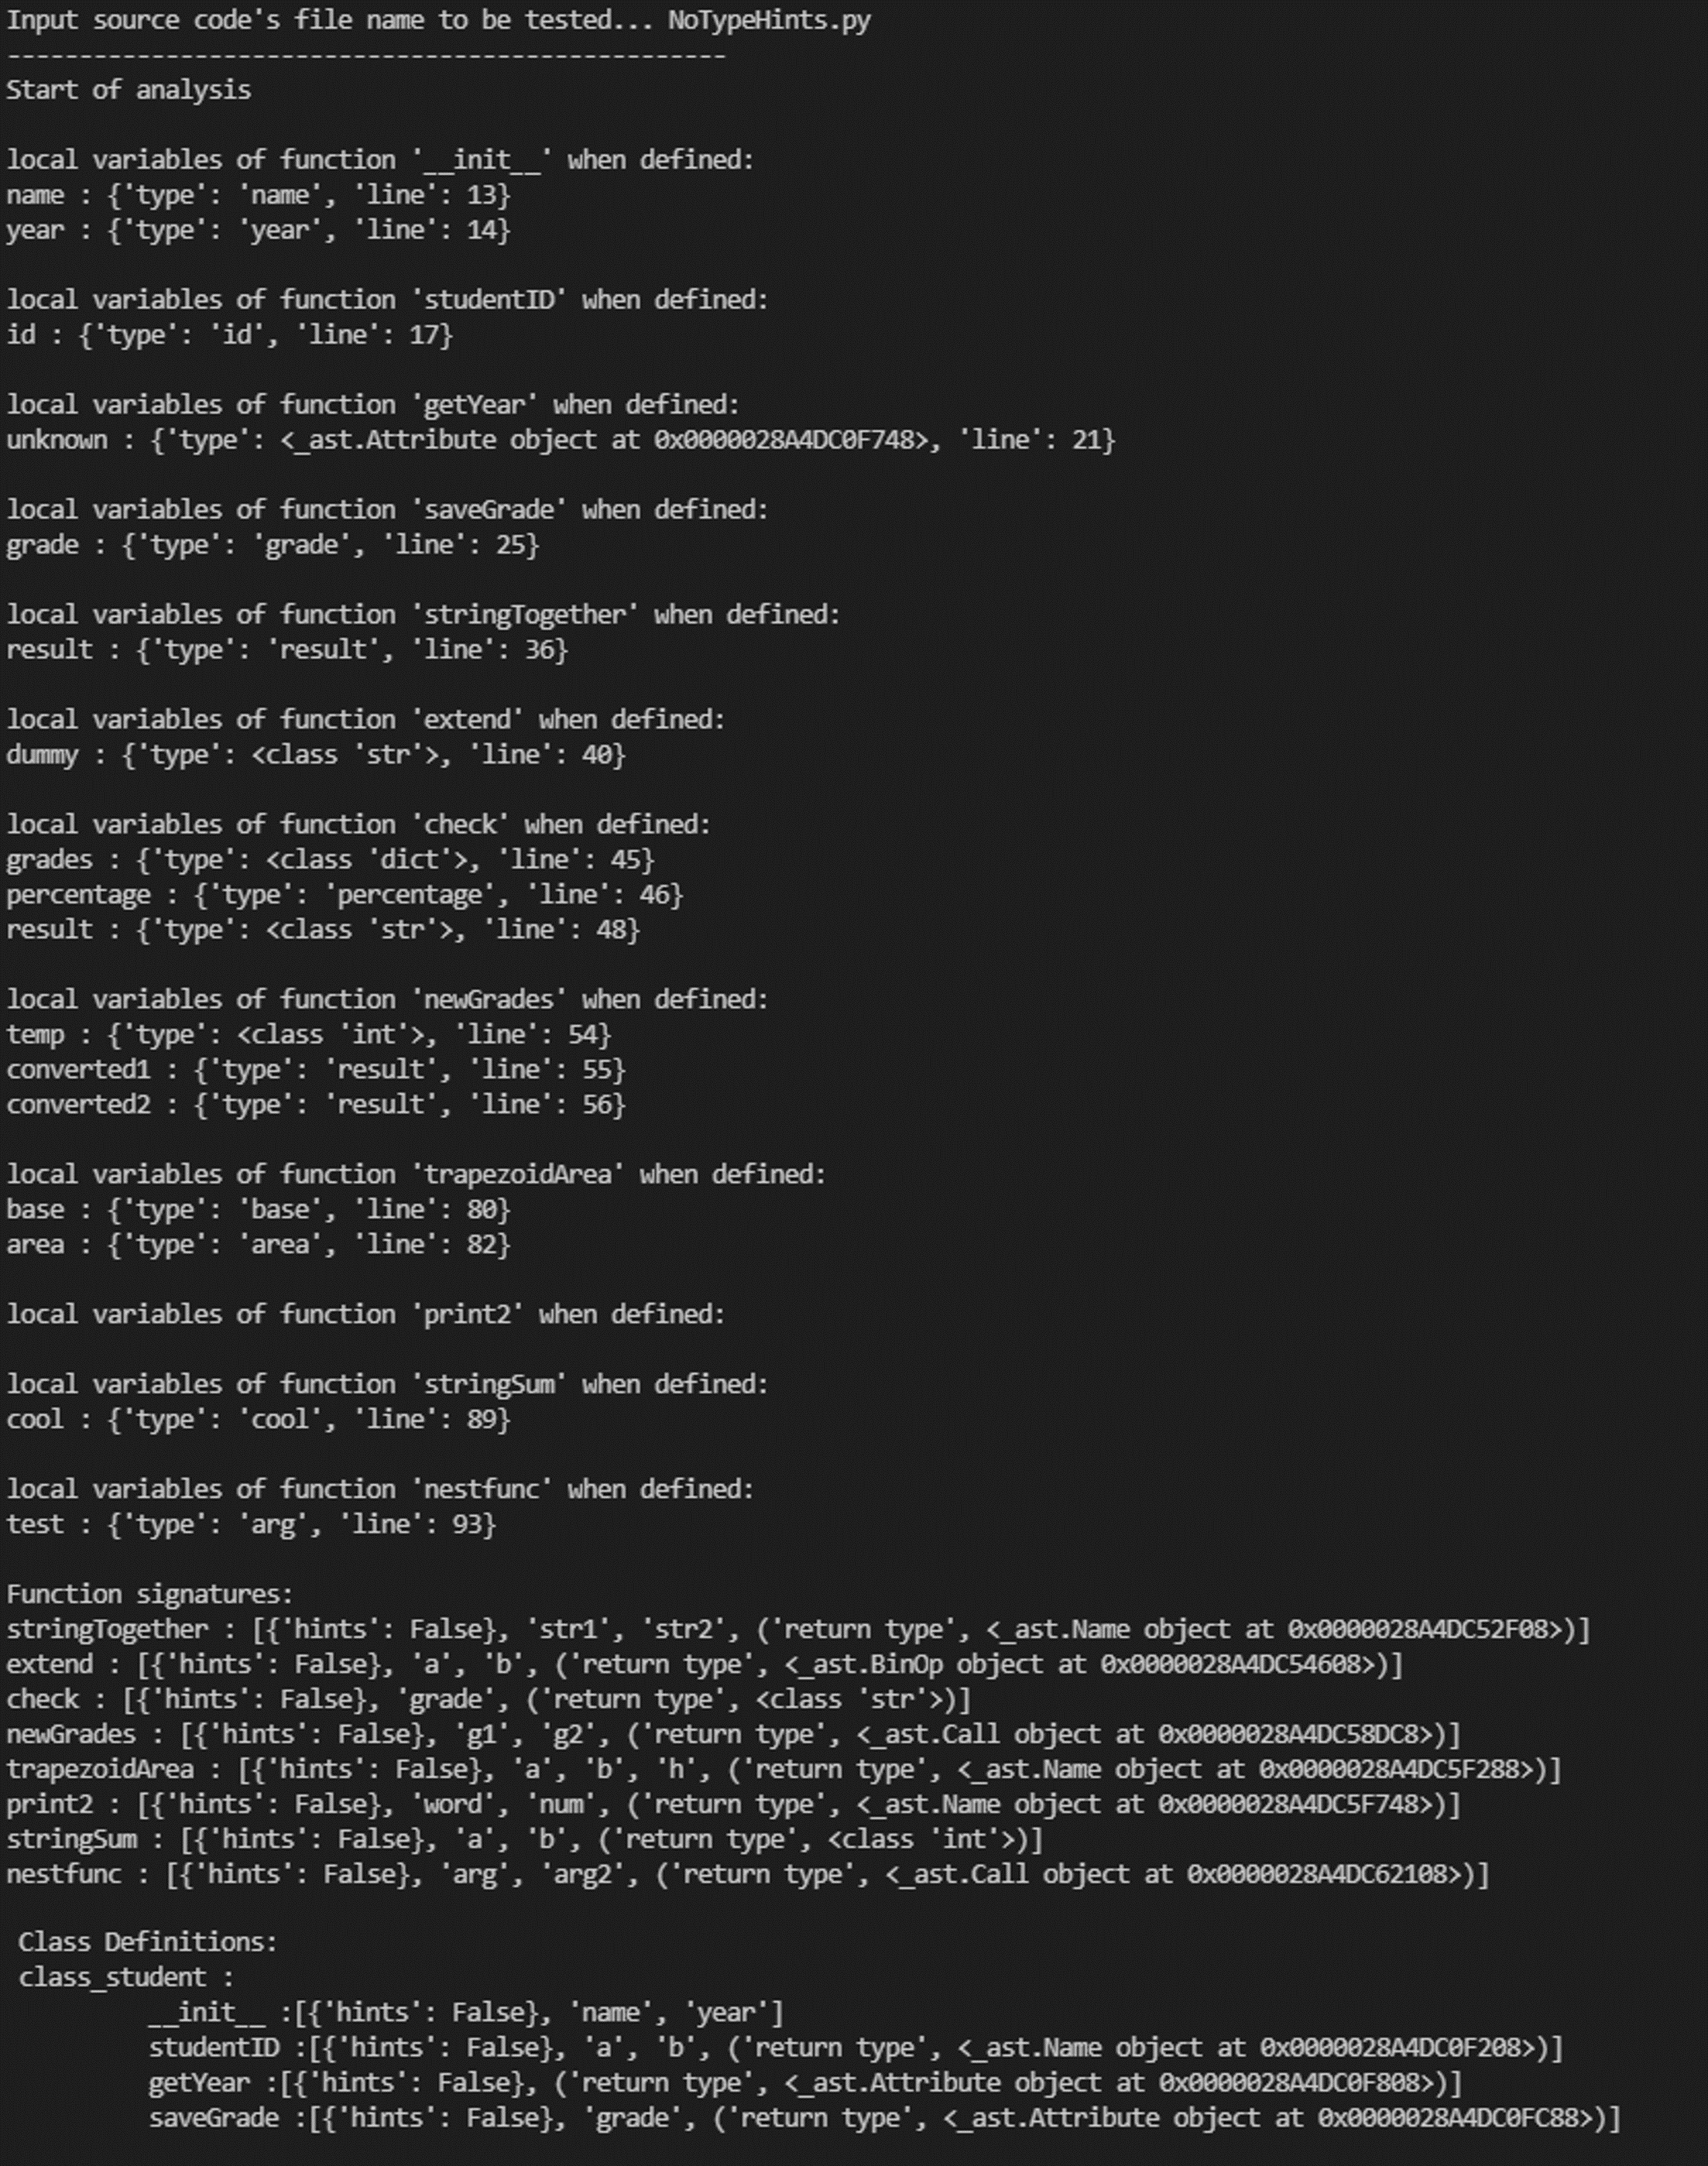
\includegraphics[width=\textwidth]{images/NoTypeHints1.png}
    \captionof{figure}{A screenshot of the first part output of the analysis of \textbf{NoTypeHints.py} produced by the static analyser}
\end{center}

\begin{center}
    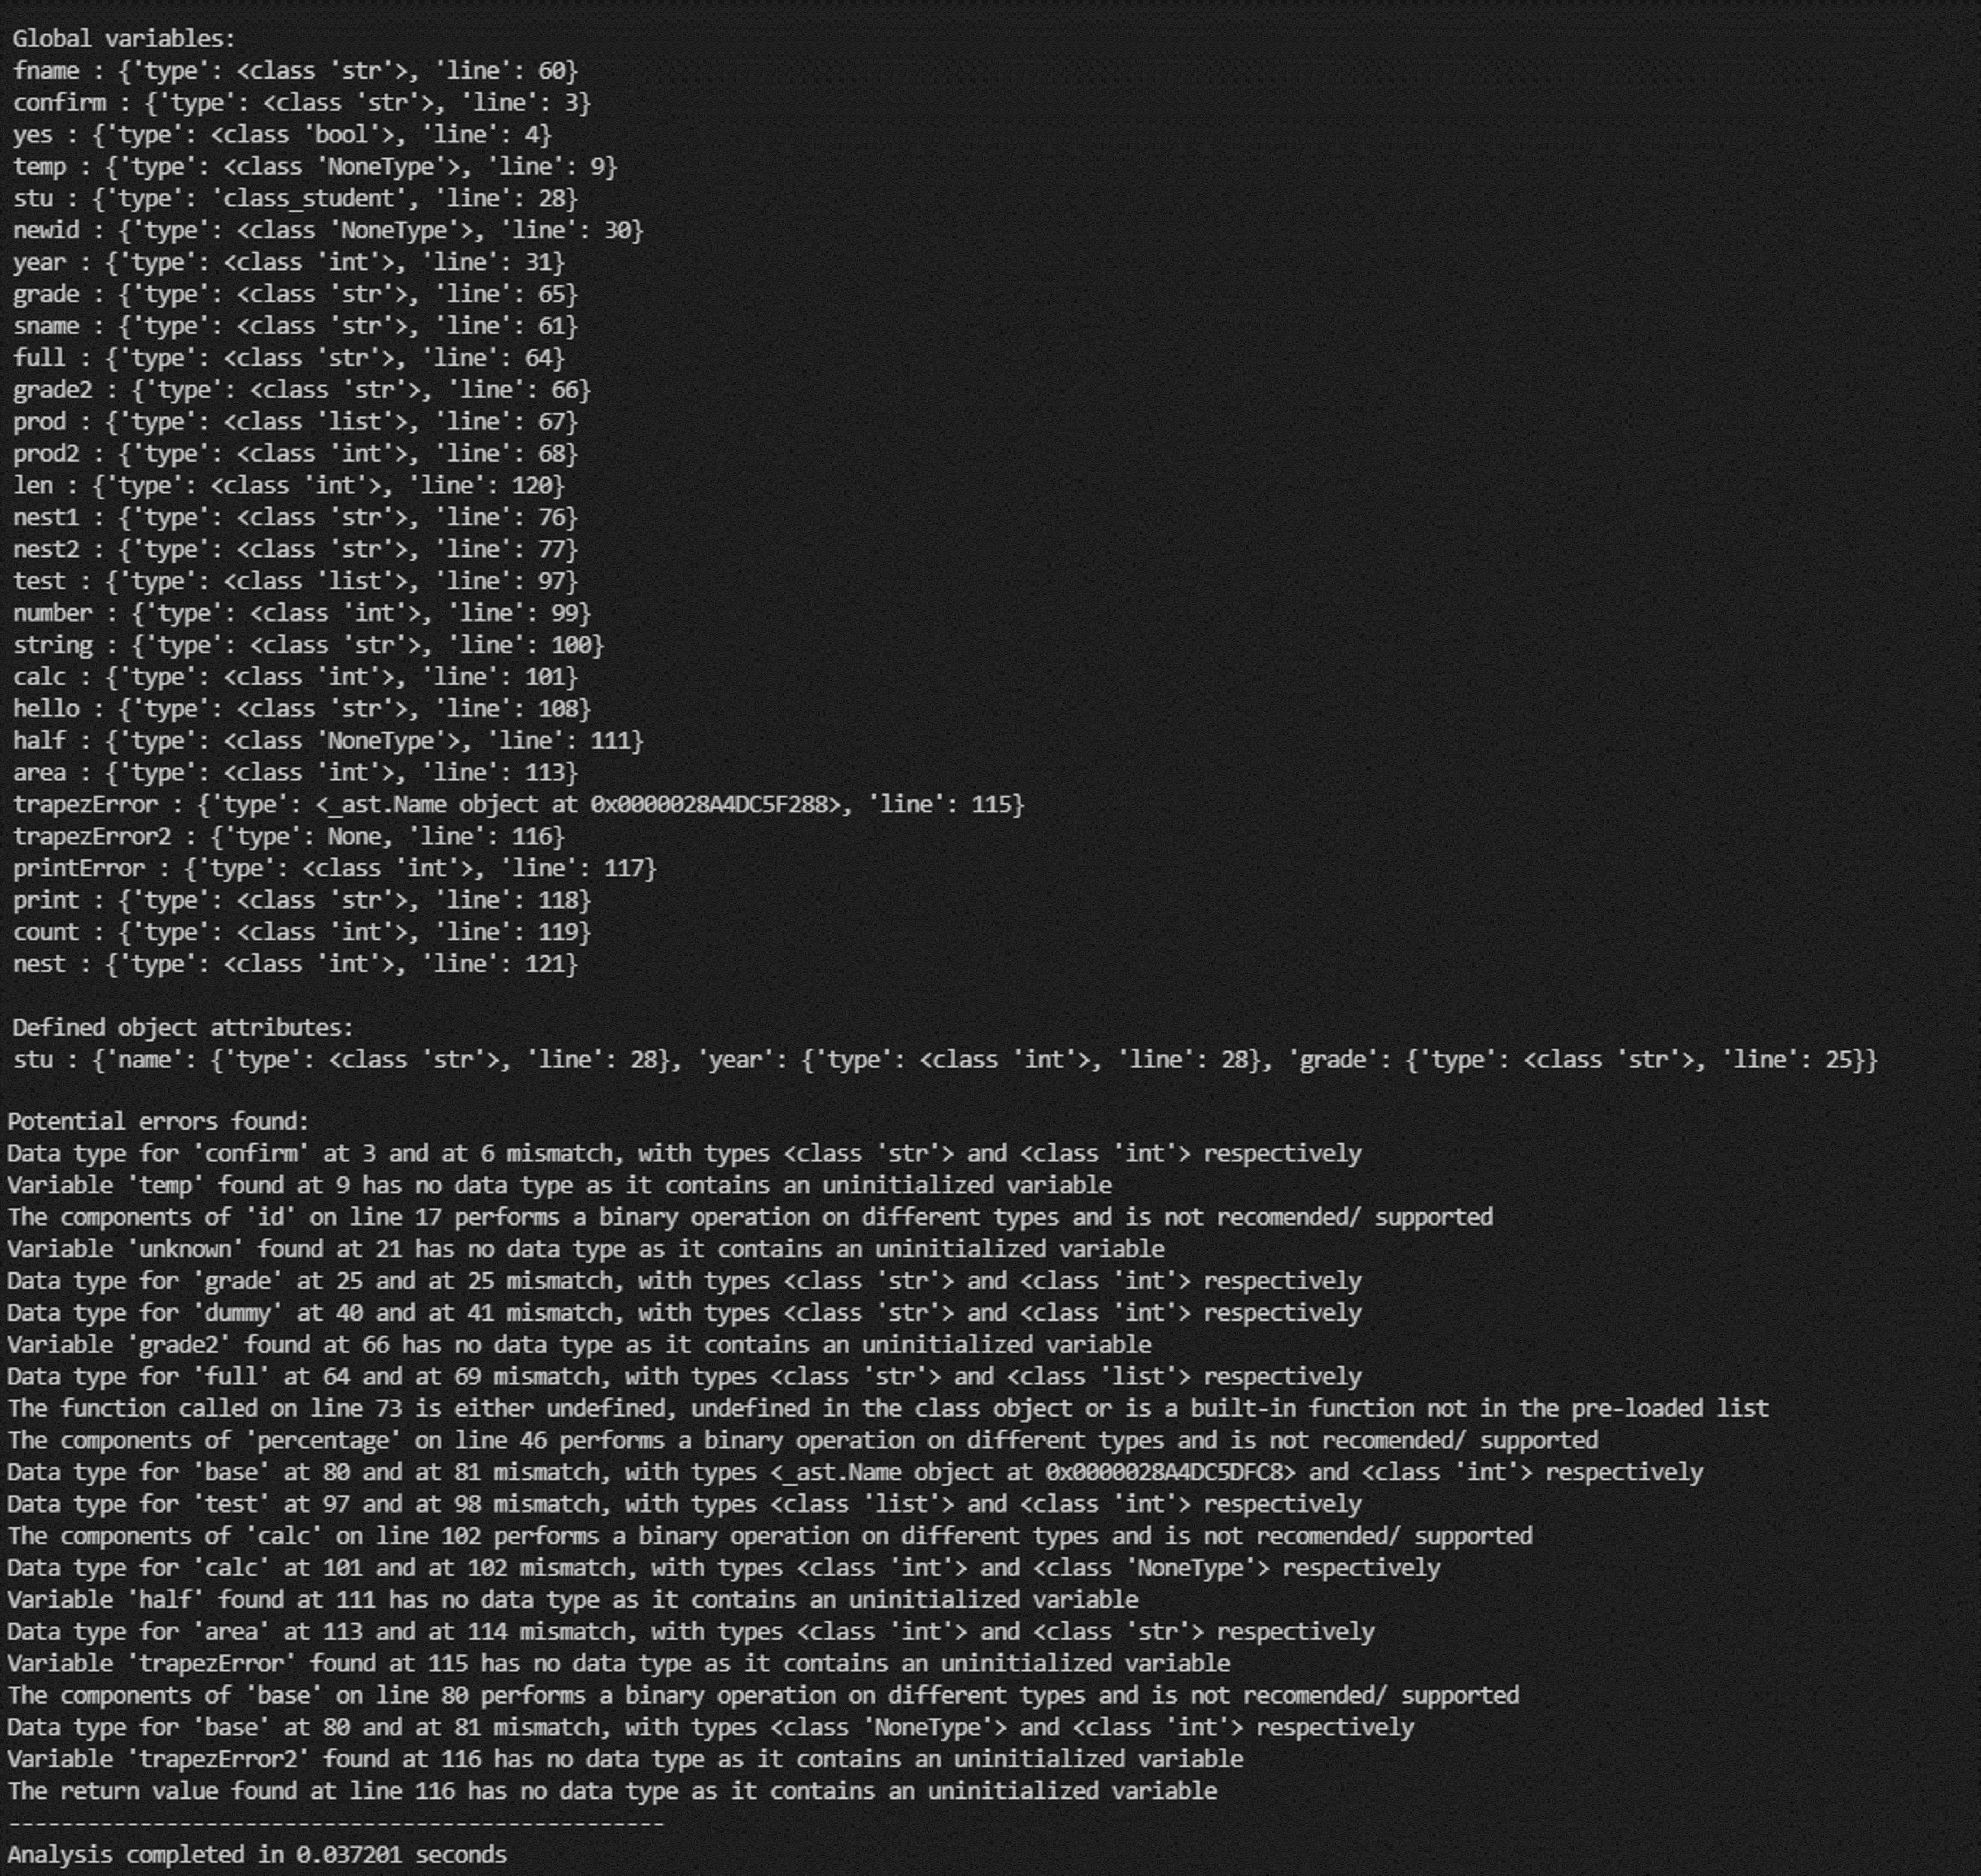
\includegraphics[width=\textwidth]{images/NoTypeHints2.png}
    \captionof{figure}{A screenshot of the second part output of the analysis of \textbf{NotypeHints.py} produced by the static analyser}
\end{center}

\begin{center}
    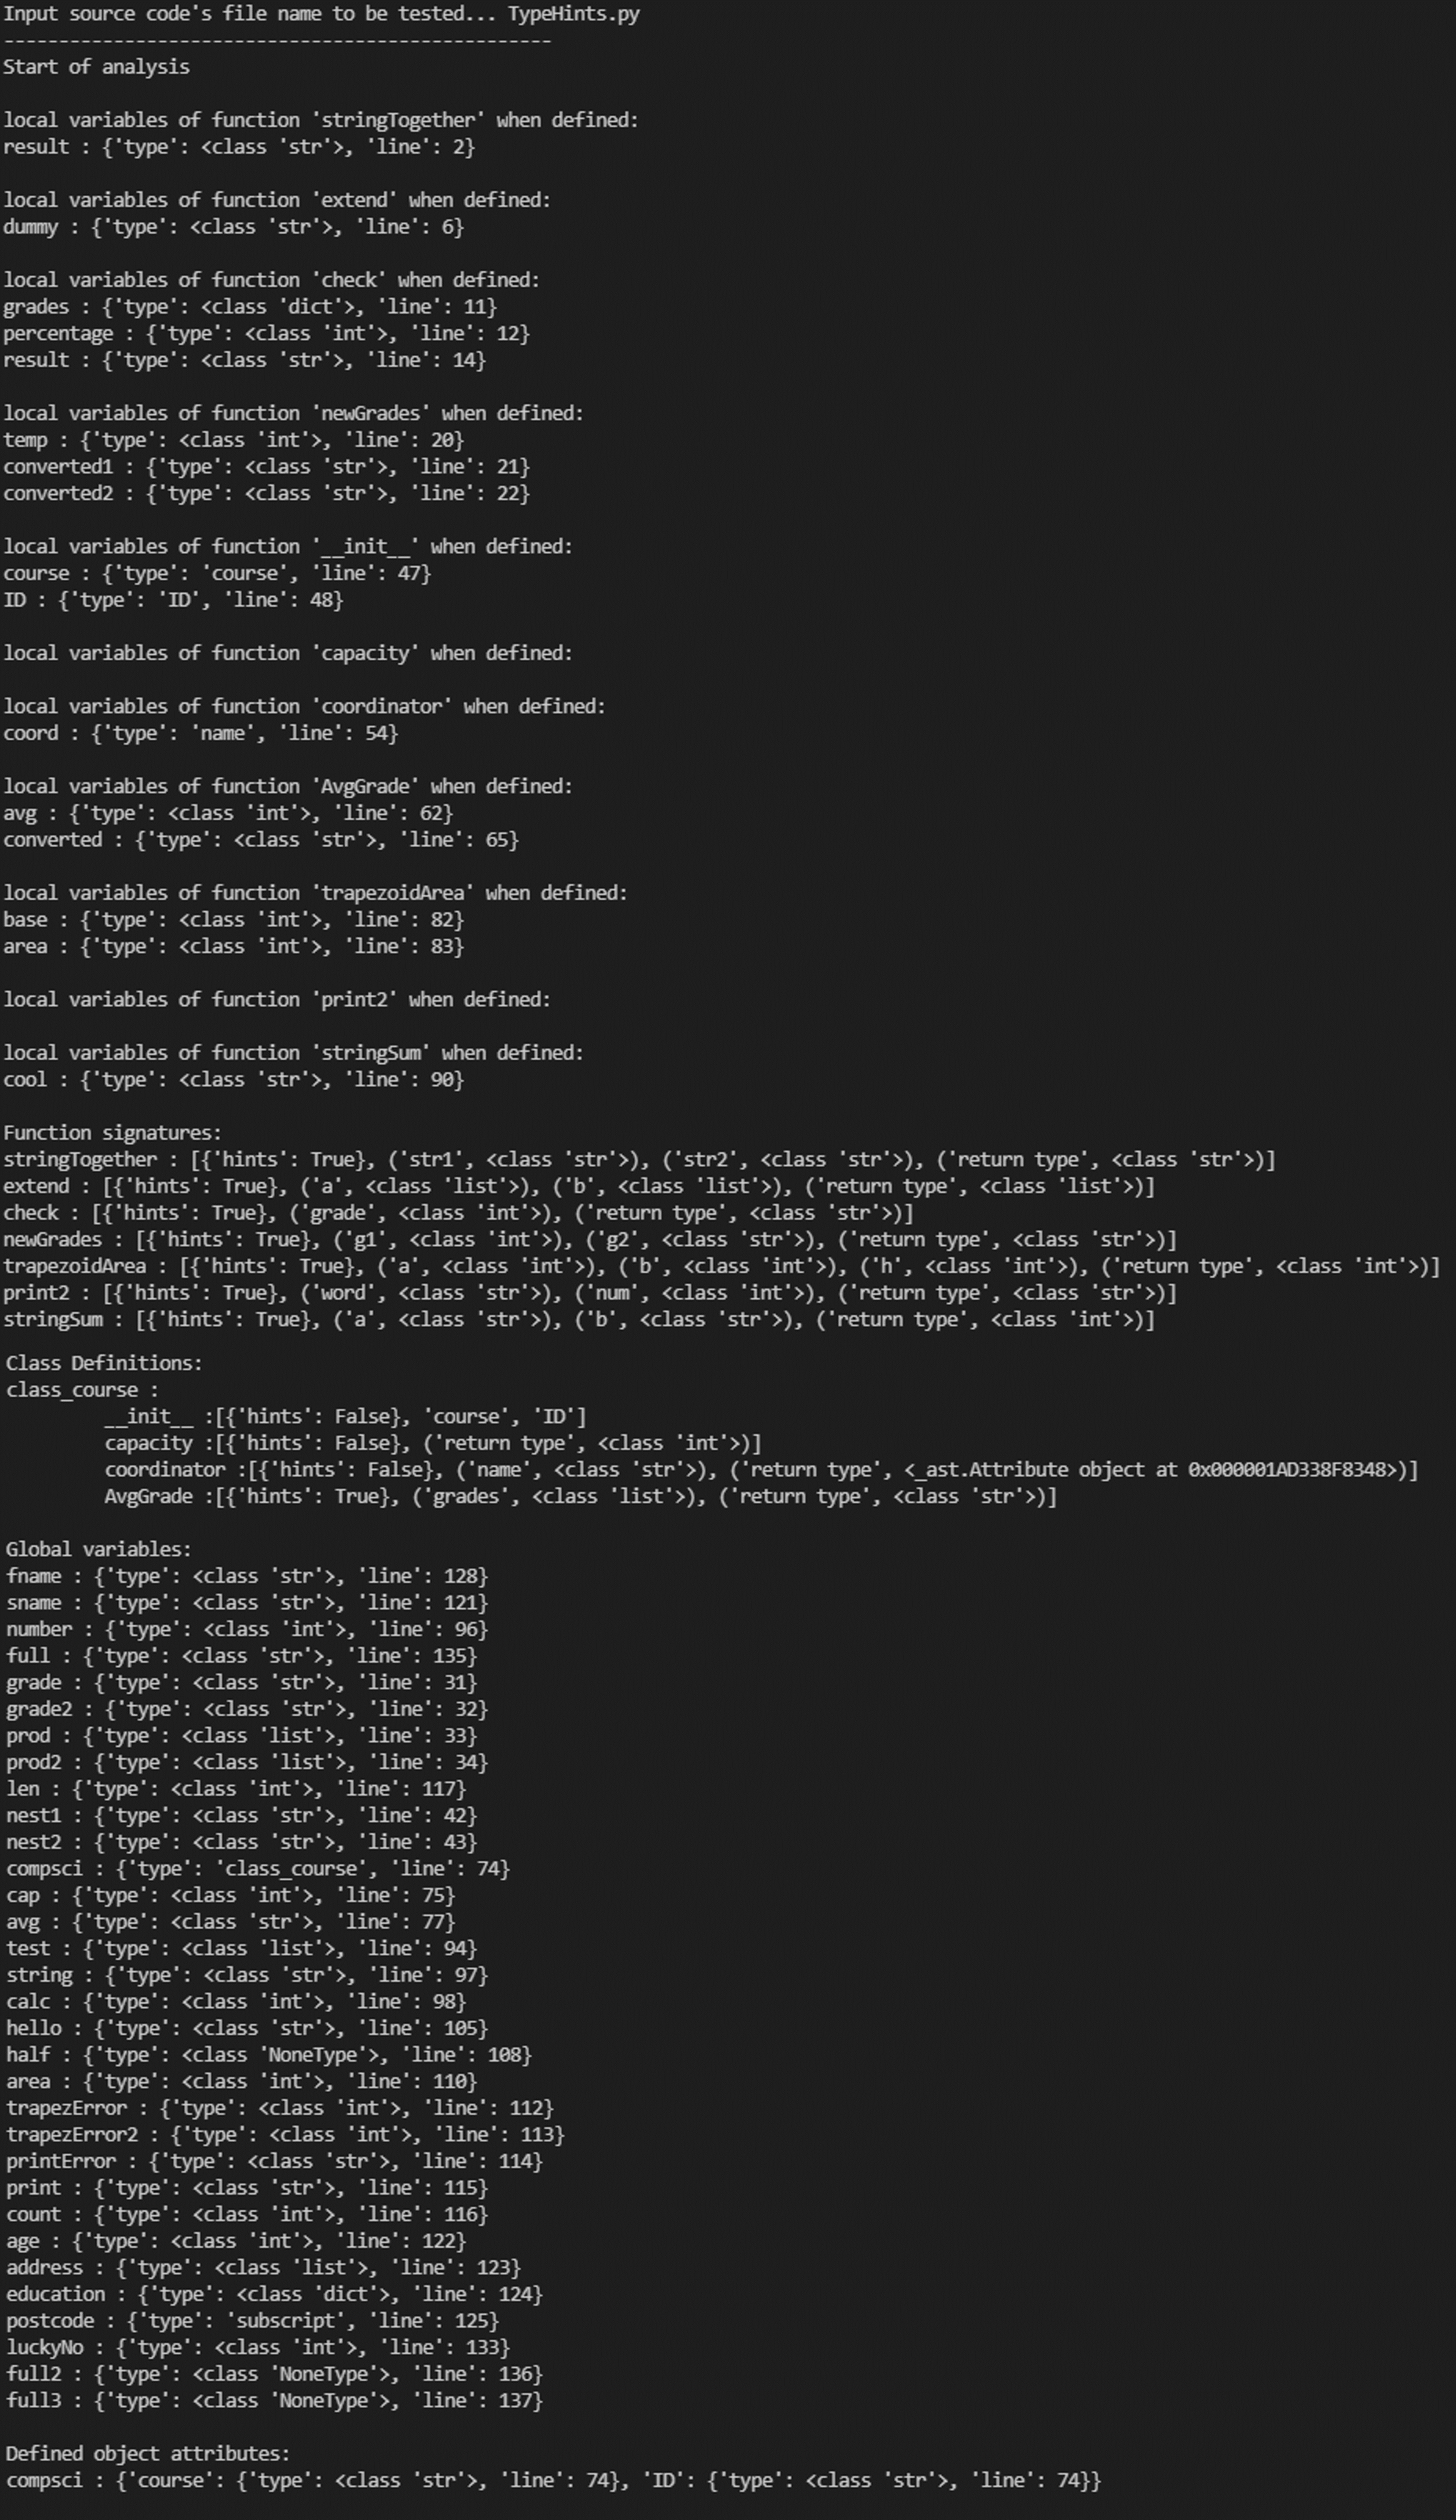
\includegraphics[width=\textwidth]{images/TypeHints1.png}
    \captionof{figure}{A screenshot of the first part output of the analysis of \textbf{TypeHints.py} produced by the static analyser}
\end{center}

\begin{center}
    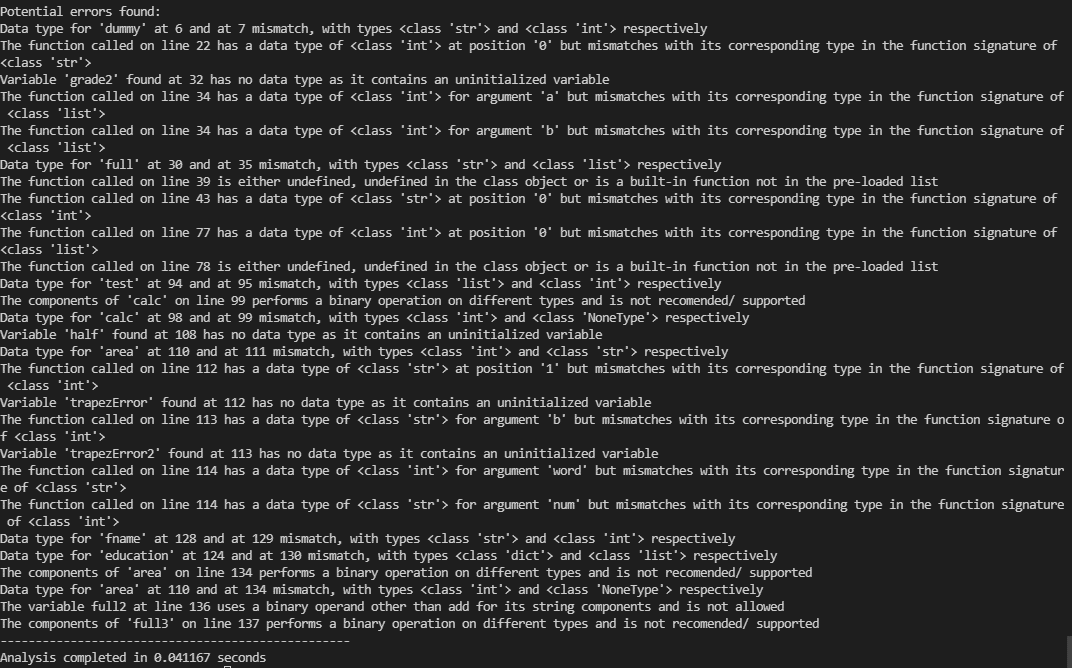
\includegraphics[width=\textwidth]{images/TypeHints2.png}
    \captionof{figure}{A screenshot of the second part output of the analysis of \textbf{TypeHints.py} produced by the static analyser}
\end{center}

\begin{center}
    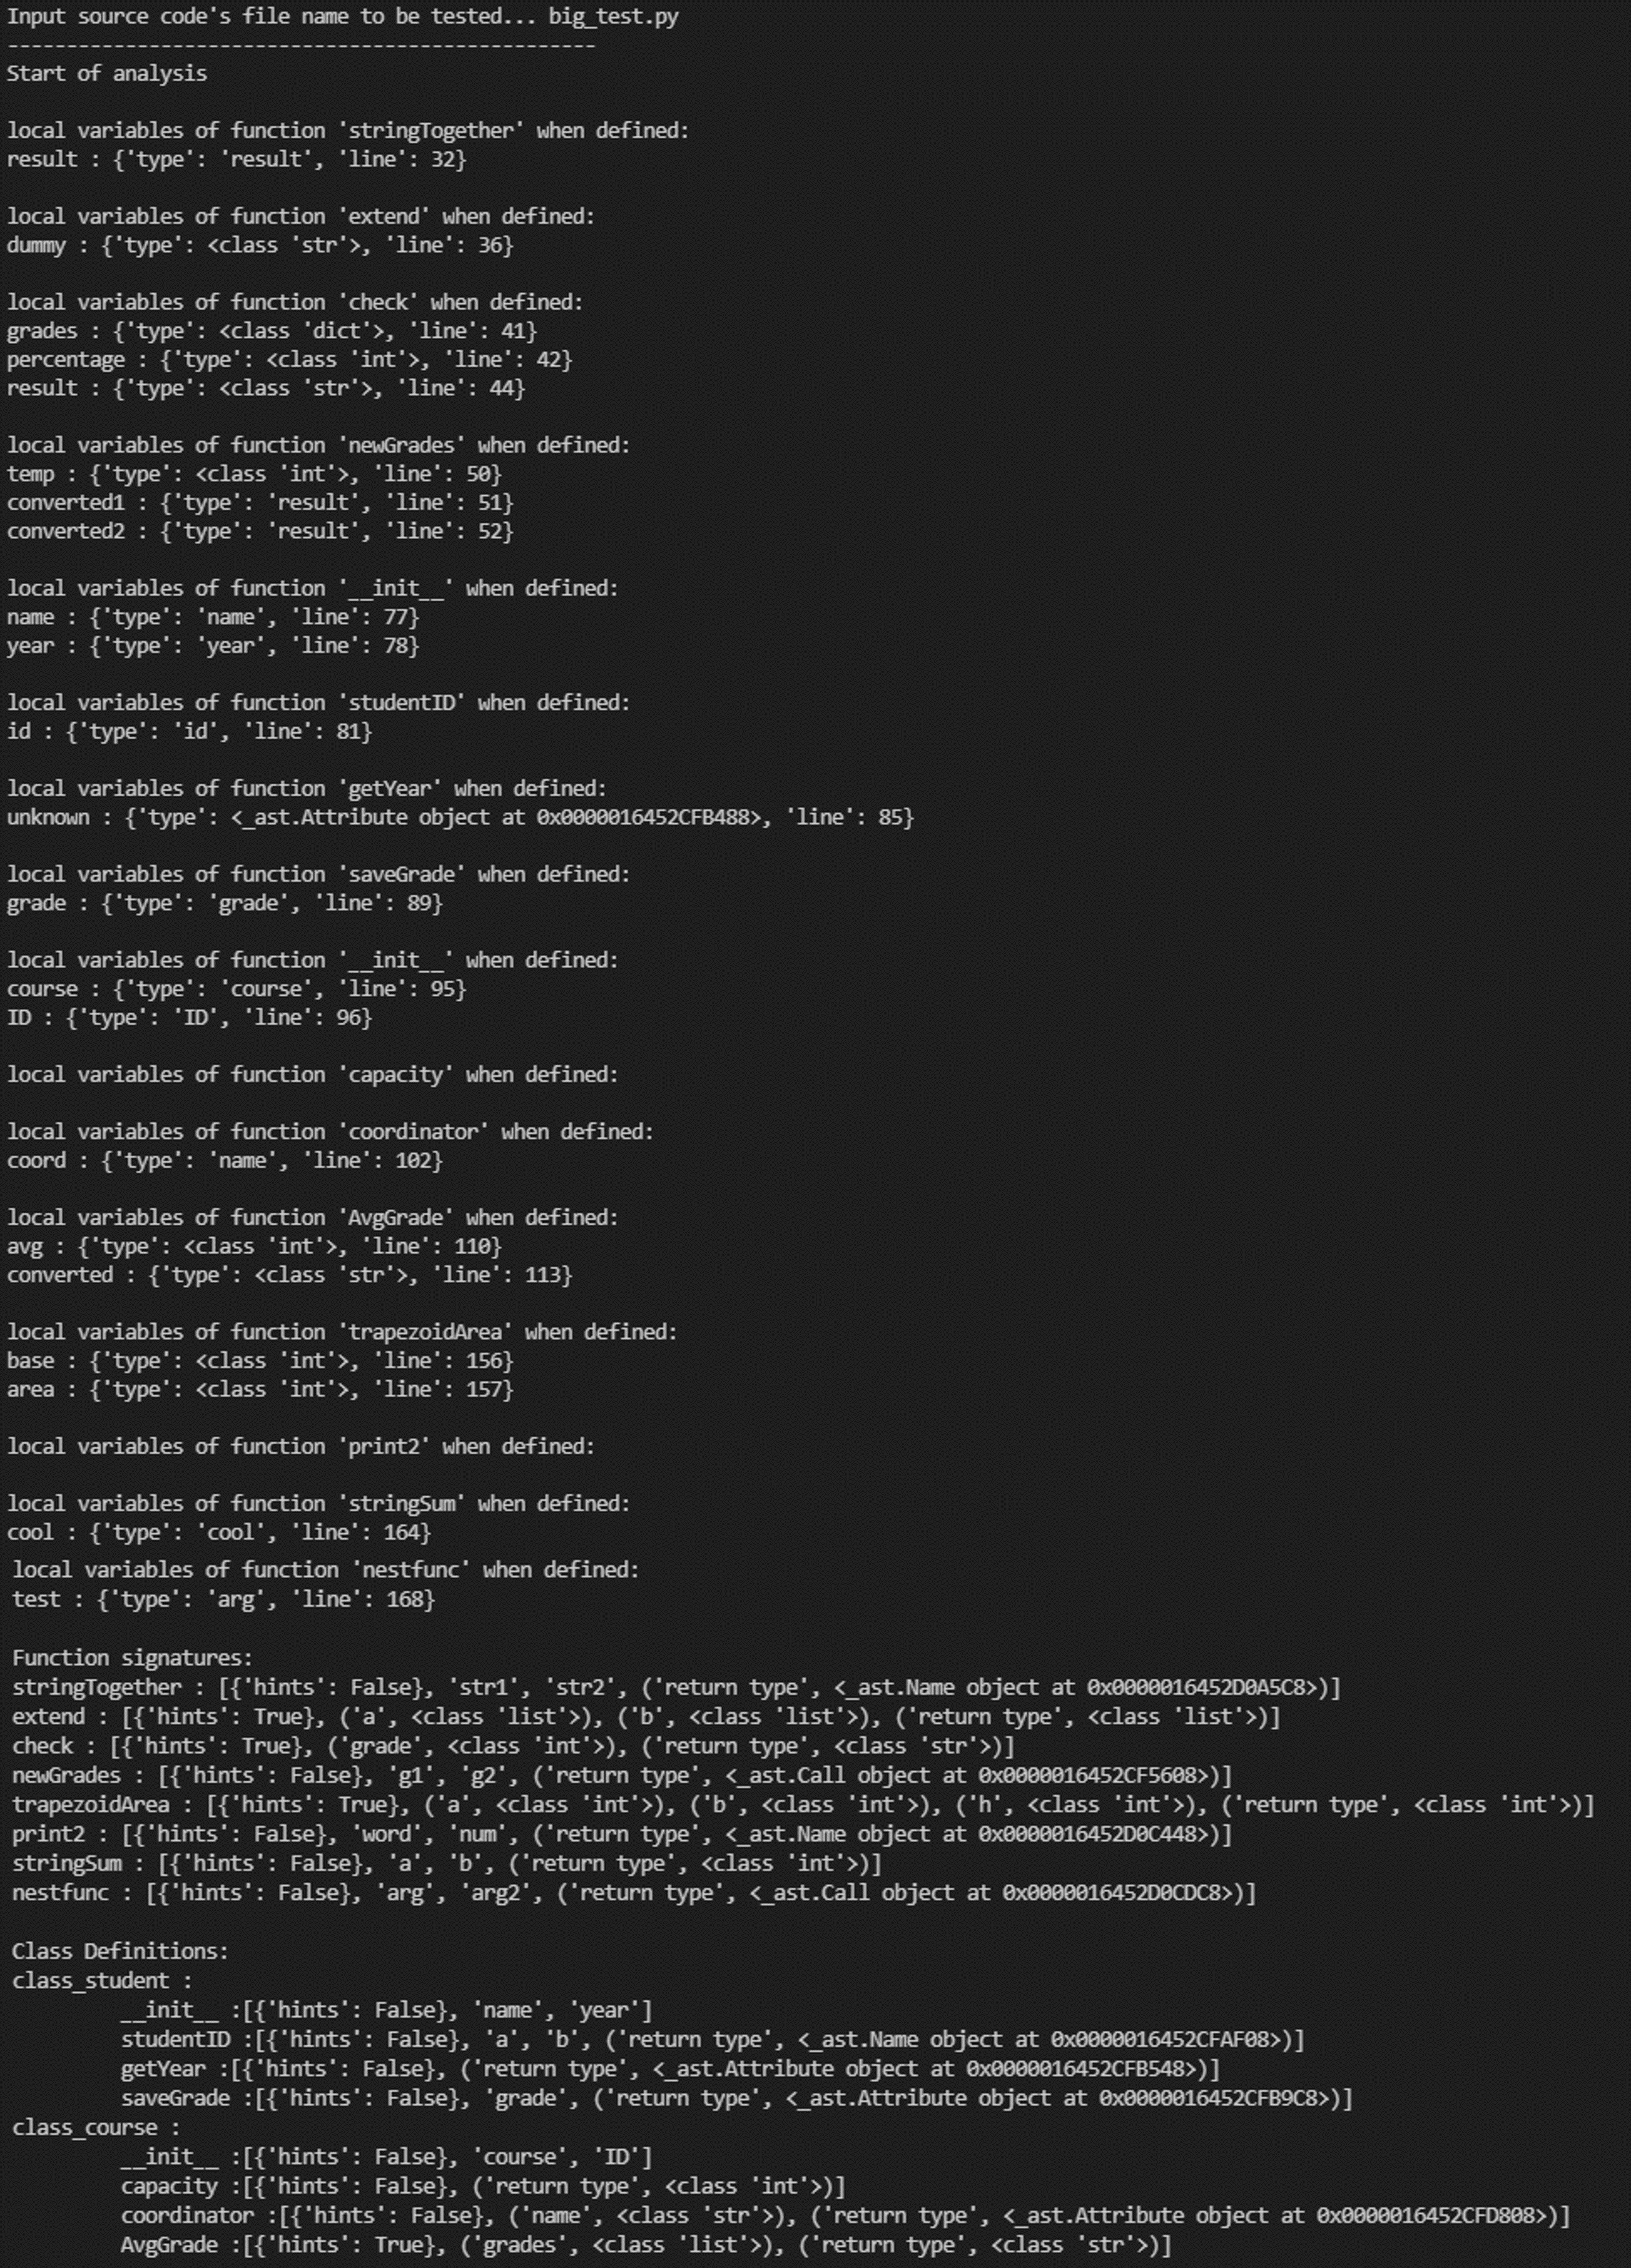
\includegraphics[width=\textwidth]{images/big1.png}
    \captionof{figure}{A screenshot of the first part output of the analysis of \textbf{big\textunderscore test.py} produced by the static analyser}
\end{center}

\begin{center}
    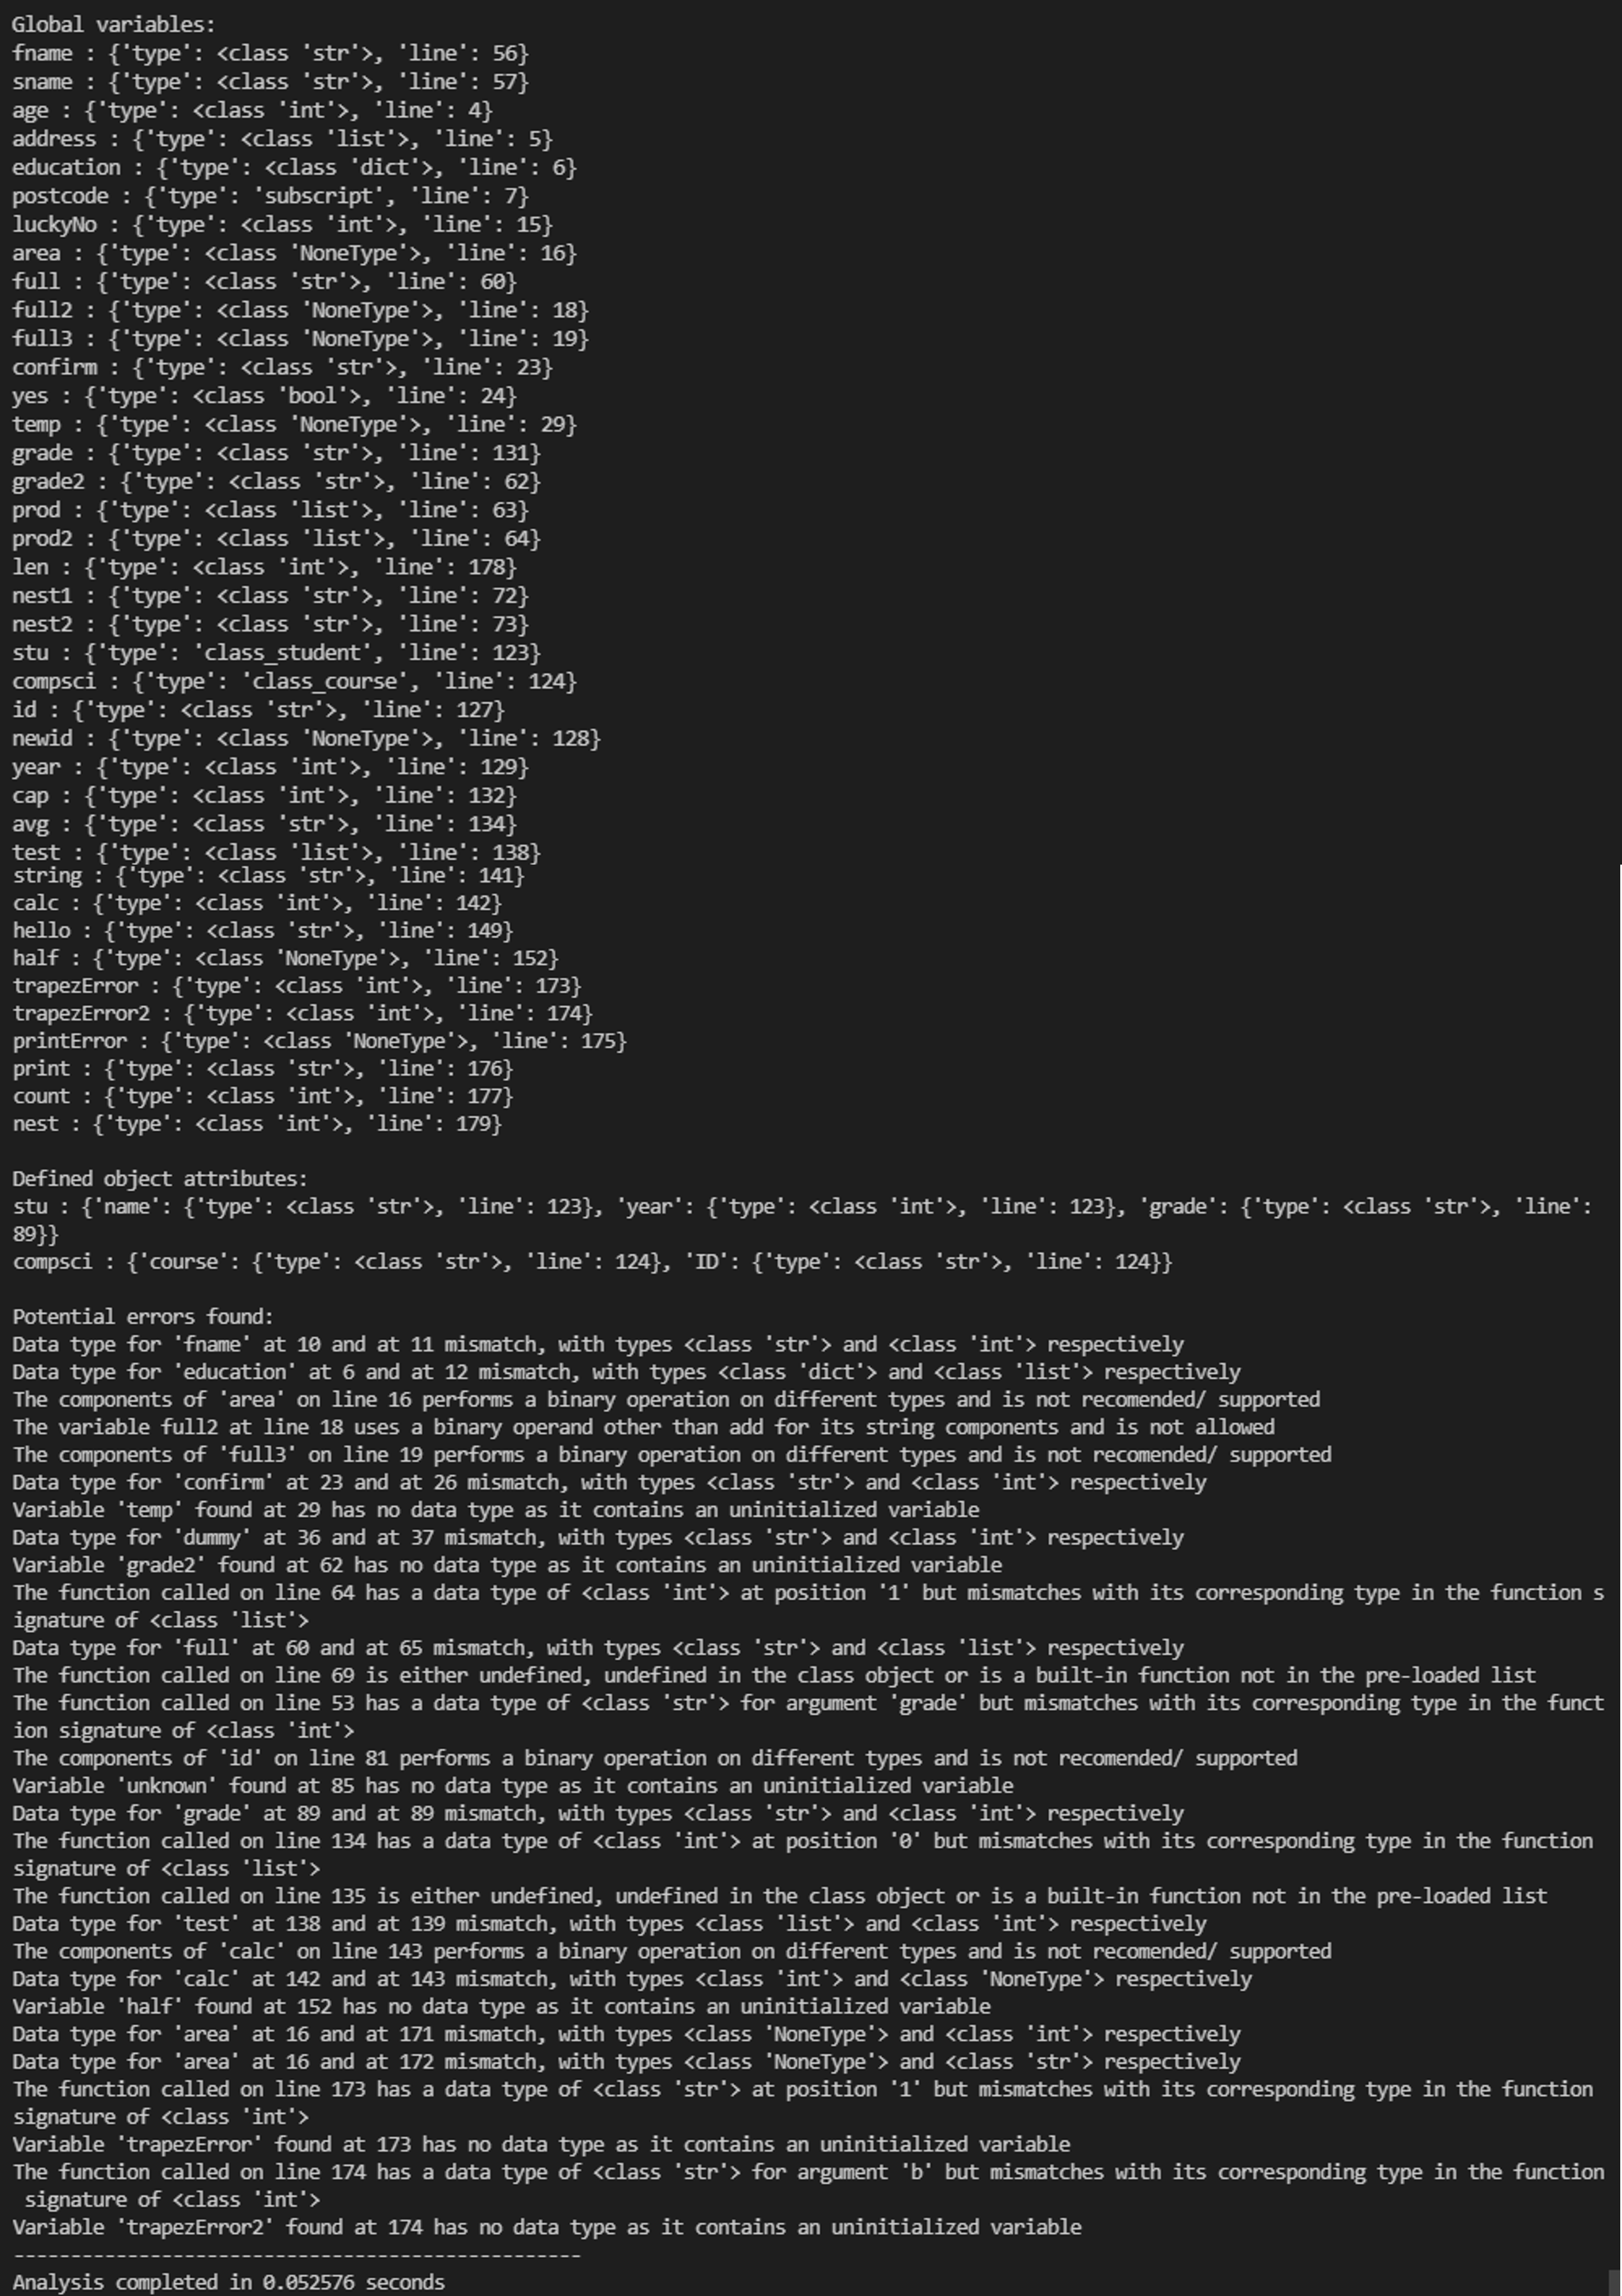
\includegraphics[width=\textwidth]{images/big2.png}
    \captionof{figure}{A screenshot of the second part output of the analysis of \textbf{big\textunderscore test.py} produced by the static analyser}
\end{center}

\section{Execution Times}
\begin{table}[h]
\begin{tabular}{|l|l|l|l|l|l|l|}
\hline
Module            & Code Size & Time 1 (ms) & Time 2 (ms) & Time 3 (ms) & Time 4 (ms) & Time 5(ms) \\ \hline
assign\_test.py   & 29        & 11.904      & 12.897      & 14.385      & 10.912      & 12.400     \\ \hline
withTH.py         & 43        & 18.849      & 14.384      & 17.360      & 15.882      & 16.368     \\ \hline
withoutTH.py      & 43        & 17.133      & 19.841      & 15.872      & 19.343      & 18.352     \\ \hline
function\_test.py & 43        & 16.863      & 16.366      & 18.351      & 14.364      & 18.352     \\ \hline
object\_test.py   & 61        & 21.825      & 21.824      & 26.289      & 25.793      & 23.807     \\ \hline
NoTypeHints.py    & 121       & 36.23       & 37.72       & 35.71       & 37.20       & 39.73      \\ \hline
TypeHints.py      & 137       & 41.66       & 41.17       & 38.19       & 35.71       & 34.22      \\ \hline
big\_test.py      & 179       & 52.576      & 35.711      & 50.591      & 45.136      & 44.640     \\ \hline
\end{tabular}
\caption{Table of the execution times the static analyser takes to analyse the module}
\label{tab:exe1}
\end{table}
\end{appendices}

%==================================================================================================================================
%   BIBLIOGRAPHY   

% The bibliography style is IEEE
% The bibliography always appears last, after the appendices.

\bibliographystyle{IEEEtran}
\bibliography{l4proj}

\end{document}
